\captionsetup[figure]{labelformat=simple, labelsep=period}
\section{Общие положения}

\subsection{Цель, объект и предмет исследования}
\begin{frame}{Цель, объект и предмет исследования}
	\textbf{Целью} работы является совершенствование методов оценки параметров гармоник мультигармонического сигнала. \vspace{1em}

	\textbf{Объектом} исследования являются методы оценки параметров гармоник в силовых электрических сетях. \vspace{1em}
	
	\textbf{Предметом} исследования является точность и быстродействие численных методов оценки параметров гармоник.	
\end{frame}

\subsection{Задачи исследования}
\begin{frame}{Задачи исследования}
	\begin{enumerate}
		\item Анализ математических основ объекта исследования и формулировка математической модели мультигармонического сигнала. Изучение и экспериментальное исследование алгоритмов оценки параметров гармоник.
		\item Развитие математической модели мультигармонических сигналов в части расчета точности оценки амплитуды применительно к используемому при оценке параметров гармоник подходу, связанному с применением оконных функций.
		\item Разработка численных методов для оценки параметров гармоник, позволяющих достичь расчетной точности для амплитуды гармоники и разработка алгоритмов для эффективного выполнения численных методов.
		\item Разработка комплекса программ для анализа и доработки алгоритмов оценки параметров гармоник мультигармонических сигналов.
	\end{enumerate}
\end{frame}

\subsection{Научная новизна работы}
\begin{frame}{Научная новизна работы}
	\begin{enumerate}
\item Расширена математическая модель спектра дискретизированного синусоидального сигнала полученными и экспериментально проверенными формулами для нахождения границы Крамера-Рао для оценки амплитуды сигнала при использовании оконной функции.
\item Предложен численный метод нахождения оптимальной несмещенной оценки параметров гармоник на основе корреляционного анализа, отличающийся тем, что позволяет оценивать параметры с теоретически максимально возможной точностью и применением быстрых алгоритмов нахождения корреляции и усеченного БПФ для повышения быстродейстия.
\item Реализован комплекс программ для экспериментальной проверки полученных в работе формул и анализа алгоритмов оценки параметров гармоник мультигармонических сигналов, отличающийся новым алгоритмом поиска гармоник и применением разработанных в работе численных методов для оценки параметров гармоник.	
\end{enumerate}	
\end{frame}

\subsection{Практическая значимость работы}
\begin{frame}{Практическая значимость работы}
	\begin{enumerate}
\item Выведена формула для нахождения границы Крамера-Рао при применении оконной функции, которая позволяет повысить эффективность научных исследований различных алгоритмов обработки сигналов с применением оконных функций, заменив моделирование алгоритма с применением различных окон расчетом по предложенной формуле.
\item Предложенный численный метод, вместе с его быстрой реализацией, позволяют повысить точность оценки параметров гармоник в различных измерительных приборах. Количественная оценка повышения точности зависит от области применения метода, для задачи оценки параметров гармоник в электрических сетях точность повышается на единицы процентов.
\item Разработанный комплекс программ позволяет проводить научные исследования в области цифровой обработки сигналов и используется в учебном процессе.	\end{enumerate}
\end{frame}

\subsection{Актуальность}
\begin{frame}{Актуальность}
Проблема точной оценки параментров гармоник рассматривается во многих отраслях науки:
\begin{tabular}{m{0.45\linewidth}m{0.45\linewidth}}
\begin{enumerate}
\item обработка сигналов;
\item биомедицина;
\item электроэнергетика;
\item адаптивное управление;
\item звуко- и радиолокация.
\end{enumerate}
\begin{figure}[ht]
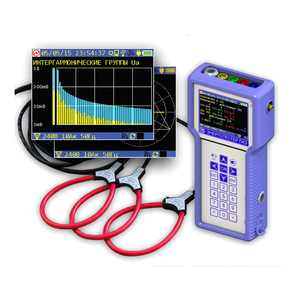
\includegraphics [scale=0.40] {ПКЭ-А.png}
\label{img:ПКЭ-А}
\end{figure}
&
\begin{figure}[ht]
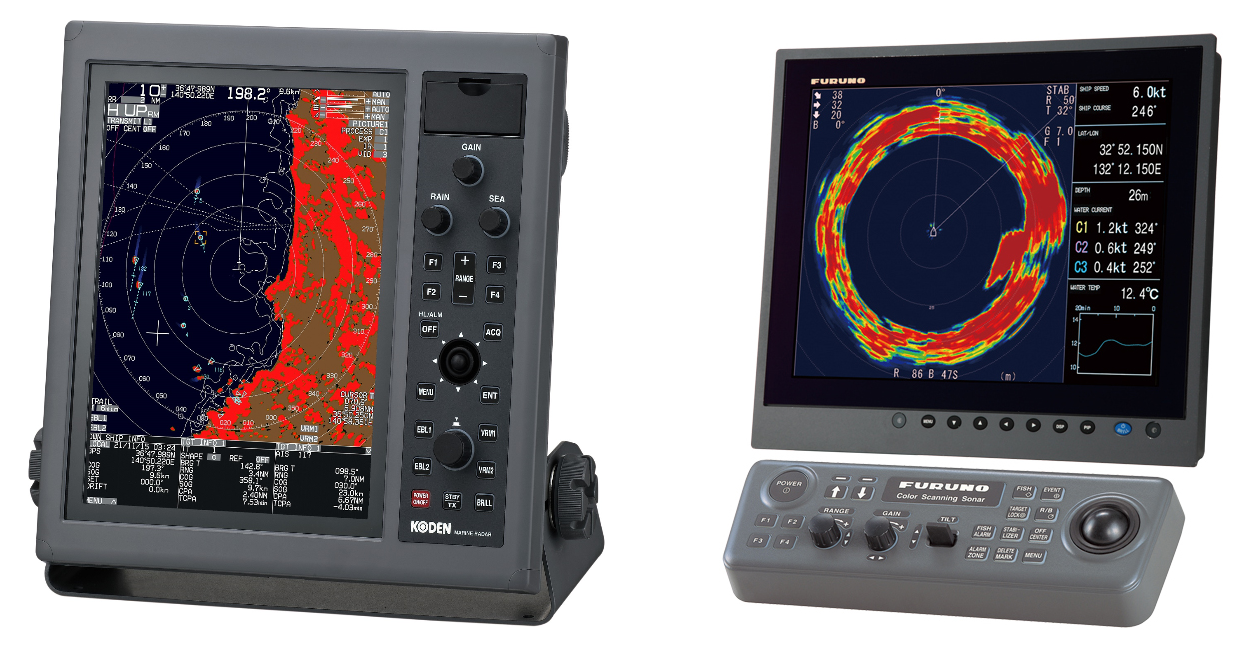
\includegraphics [scale=0.16] {Radar_Sonar.png}
\label{img:sonar}
\end{figure}
\begin{figure}[ht]
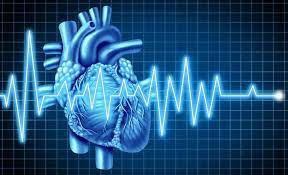
\includegraphics [scale=0.43] {heart.jpeg}
\label{img:heat}
\end{figure}
\end{tabular}
\end{frame}

\section{Математическая модель мультигармонического сигнала}
\subsection{Ограничение ДПФ}
\begin{frame}{Ограничение ДПФ}
\begin{tabular}{m{0.5\linewidth}m{0.5\linewidth}}
\textbf{Модель сигнала}:	
\begin{equation}
\label{eq:equation1}
\mathrm{s(t)} = \displaystyle\sum_{k=0}^{N-1} A_k \cos \left({\frac{2 \pi}{T_s} f_{peak} t  + \varphi_k} \right)+ \eta(t)  
\end{equation}
\textbf{ДПФ}:		
\begin{equation}
\label{eq:equation3}
	\dot{X}(k)= \displaystyle\sum_{k=0}^{N-1} x(n) \cdot \exp\left( -j \cdot \frac{2 \pi n k}{N}\right)
\end{equation}  
%при $k=0,1, \cdots > N - 1$
&
\begin{figure}[ht]
%\centering
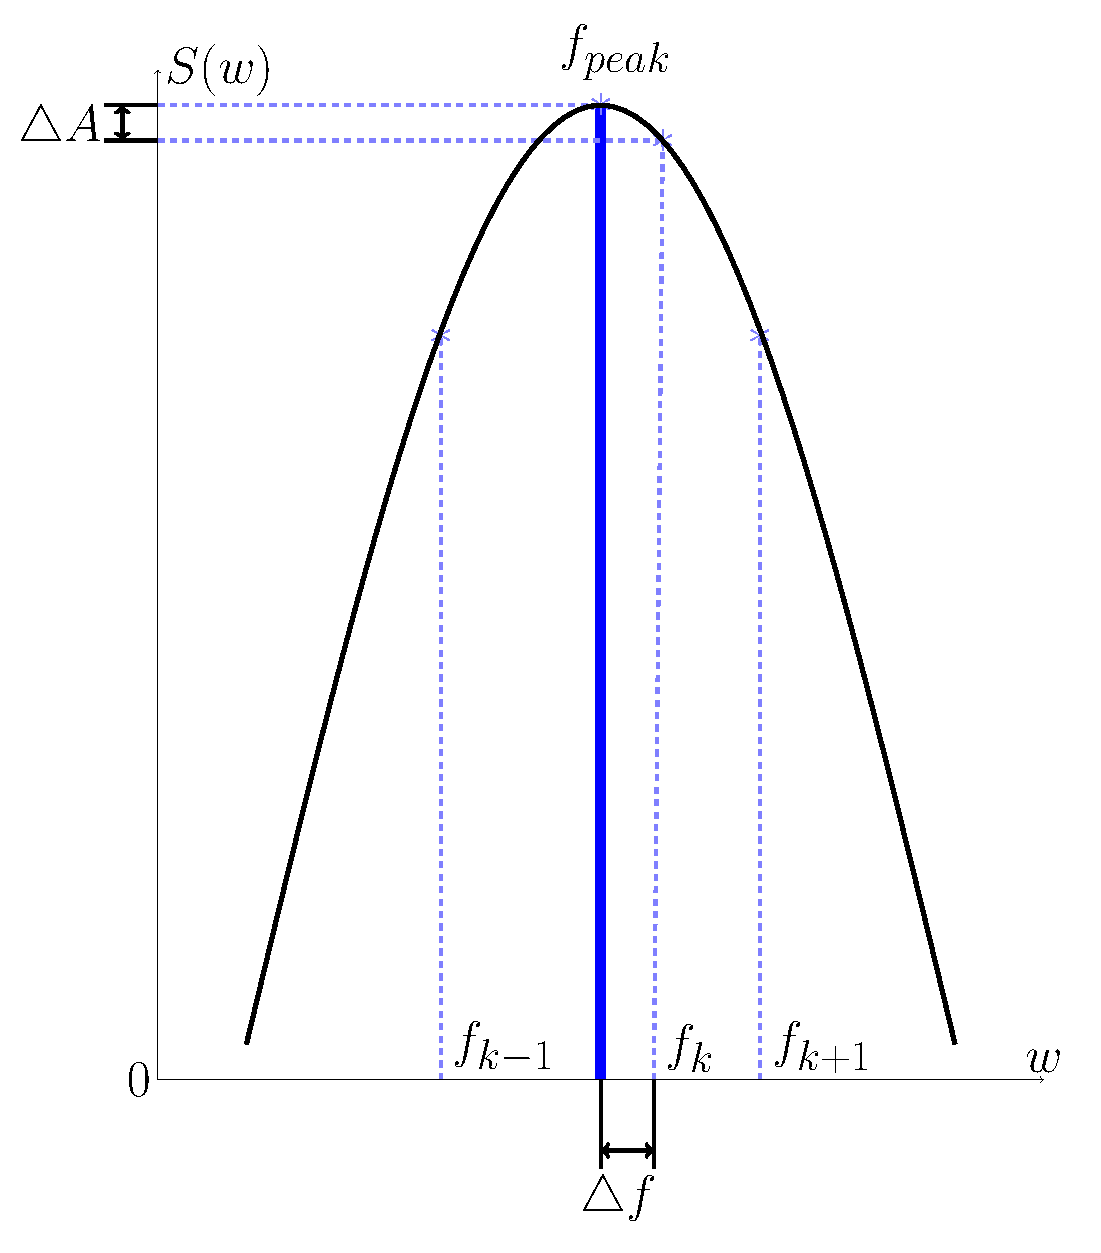
\includegraphics [scale=0.27] {Maximum_DFT.pdf}
\begin{flushright}
\caption{Случай несовпадения максимума ДПФ и максимума спектра гармоник.}	
\end{flushright}
\label{img:picture1}
\end{figure}
\end{tabular}
% E. Jacobsen and P. Kootsookos, "Fast, Accurate Frequency Estimators [DSP Tips & Tricks]," in IEEE Signal Processing Magazine, vol. 24, no. 3, pp. 123-125, May 2007, doi: 10.1109/MSP.2007.361611.
%Jacobsen E. On local interpolation of DFT outputs //Available online: http://www. ericjacobsen. org/FTinterp. pdf.[Accessed January 2013]. – 1994.
\end{frame}

\begin{frame}{Влияние оконной функции}
%	\textsc{Рисунок, показывающий, что происходит со спектром гармоники при наложении на него окна. Лучше в двух частях - с прямоугольным окном и окном Кайзера.}	
\begin{minipage}[t]{0.47\linewidth}
	\centering 
	\textbf{Прямоугольное окно}
	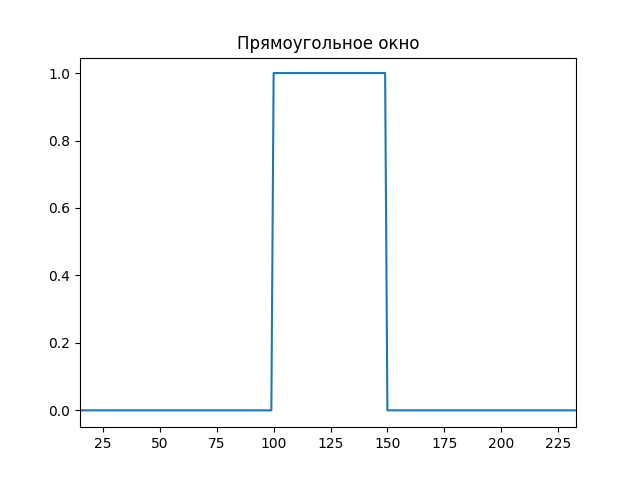
\includegraphics[width=.85\linewidth]{Прямоугольное окно240521.png}
	\textbf{Окно Кайзера}
	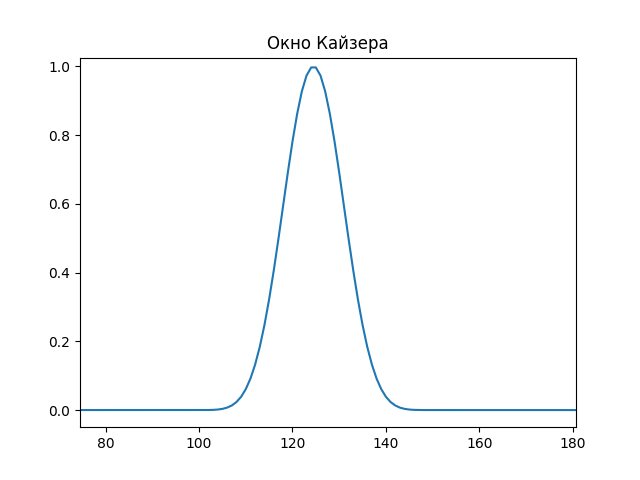
\includegraphics[width=.85\linewidth]{ОкноКазера240521.png}		
\end{minipage}
\hfill
\begin{minipage}[t]{0.47\linewidth}
	\centering 
	\textbf{Спектр с прям-ым окном}
	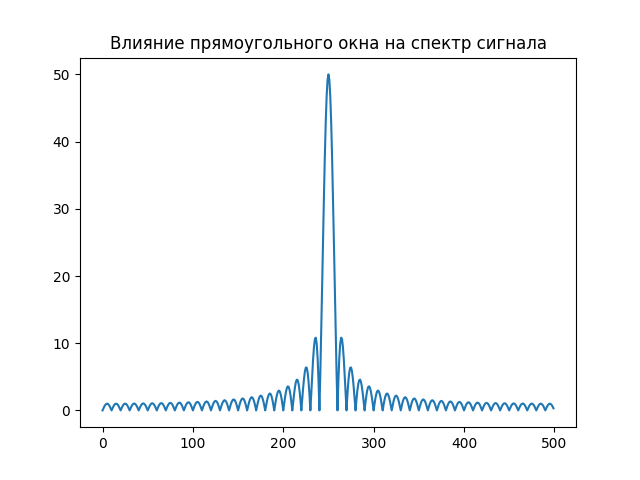
\includegraphics[width=.85\linewidth]{ПрямоугольныйСпект230421.png}
	\textbf{Спектр с окном Кайзера}
	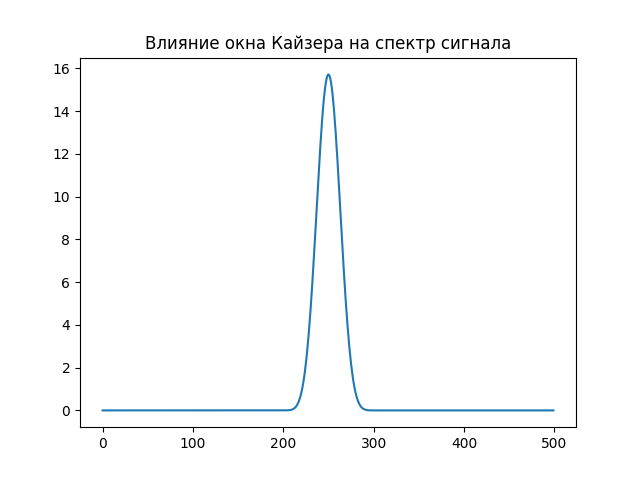
\includegraphics[width=.85\linewidth]{СпектрОкняКайзера230421.png}
\end{minipage}
\end{frame}

\begin{frame}{Методы интерполирования спектра}
\begin{tabular}{m{0.45\linewidth}m{0.45\linewidth}}
\small{
\begin{itemize}	
	\item Метод Якобсена;
	\item Два метода Квина;
	\item Два метода Маклеода;
	\item Метод Грэндка;
	\item Алгоритм параболической интерполяции;
	\item Алгоритм интерполяции Гаусса;
	\item Алгоритм, рекомендованный в ГОСТ 30804.4.7-2013;
	\item Метод корреляционных функций;
	\item Модернизированный метод корреляционных функций.				
\end{itemize}}
&	
%\textbf{Разность между дискретными гармониками:}
\begin{equation}
	\label{eq:equation2}
	\bigtriangleup f = \frac{(|X_{k+1}|-|X_{k-1}|)}{(4|X_{k}|-2|X_{k-1}|-2|X_{k+1}|)}
\end{equation}

\begin{equation}
	\label{eq:equation7}
	f_{peak} = f_k + \bigtriangleup f
\end{equation}
\begin{equation}
	\label{eq:equation8}
	f_{tone} = f_{peak} \cdot \frac{f_s}{N}
\end{equation}
%\begin{equation}
%	\label{eq:equation4}
%	u(f_k-1) = a \cdot (f_k-1-\bigtriangleup f)^2 + b
%\end{equation}
%\begin{equation}
%	\label{eq:equation5}
%	u(f_k) = a \cdot (f_k-\bigtriangleup f)^2+b,
%\end{equation}
%\begin{equation}
%	\label{eq:equation6}
%	u(f_k+1) = a\cdot (f_k+1-\bigtriangleup f)^2 +b
%\end{equation}
\end{tabular}
\end{frame}

\begin{frame}{Методы экстраполирования сигнала}
	\begin{minipage}[t]{0.45\linewidth}
		\centering 
		\textbf{Сигнал (частота=5.2)}
		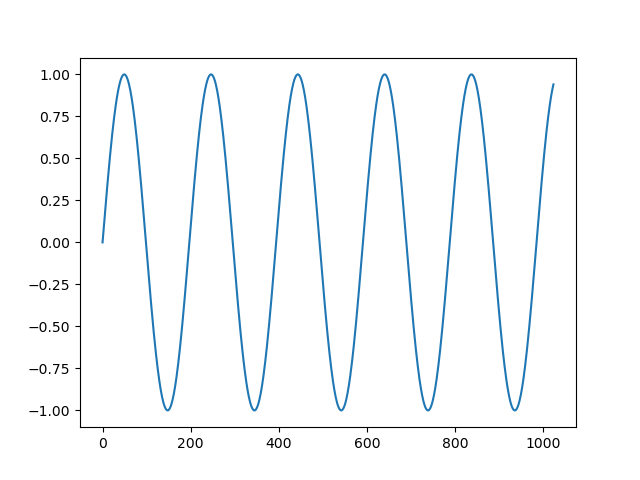
\includegraphics[width=.85\linewidth]{signal}
		\textbf{Экстраполированный сигнал }
		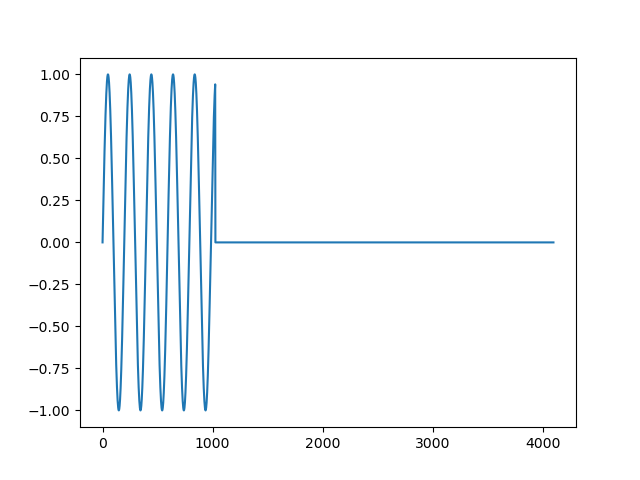
\includegraphics[width=.85\linewidth]{interpolated_signal}		
	\end{minipage}
	\hfill
	\begin{minipage}[t]{0.45\linewidth}
		\centering 
		\textbf{Спектр}
		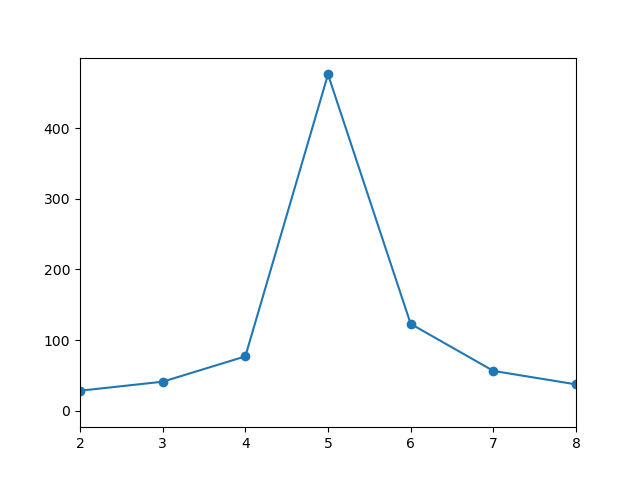
\includegraphics[width=.85\linewidth]{spectrum}
		\textbf{Спектр экстр. сигнала}
		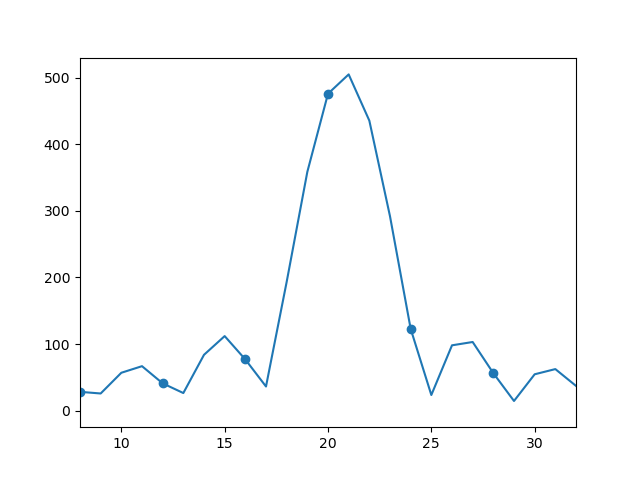
\includegraphics[width=.85\linewidth]{spectrum_of_interpolated_signal}
	\end{minipage}
\end{frame}

\subsection{Граница Крамера-Рао}
\begin{frame}{Общая формула границы Крамера-Рао}
%Теоретическая точность определения амплитуды гармоник	
\begin{tabular}{m{0.45\linewidth}m{0.45\linewidth}}
\textbf{Граница Крамера-Рао:}
\begin{equation}
\label{eq:equation13}
var(\theta)\geq \frac{1}{I(\theta)}
\end{equation}
$\theta$ – оцениваемый параметр;
		
$var(\theta)$ – дисперсия (variance) несмещенной оценки параметра.

\textbf{Информация Фишера:}
\begin{equation}
	\label{eq:equation14}
	I(\theta) = -E \left[\frac{\delta^2 ln p(x;\theta)}{\delta\theta^2}\right]
\end{equation}
где $E$ – среднее значение;

$p(x;\theta)$ – функция правдоподобия.
&
\textbf{Общая оценка границы Крамера-Рао для сигналов в белом Гауссовом шуме:}
\begin{equation}
	\label{eq:equation14}
x[n] = s[n;\theta] + w[n], n=0,1,...,N-1	
\end{equation}
$x[n]$ -- векторный параметр;

$\theta$  -- оцениваемый параметр;

$w[n]$ -- белый Гауссовый шум;

$s[n;\theta]$ -- детерминированный сигнал.
\begin{equation}
\label{eq:equation14}
var(\hat{\theta}) \geq \frac{\sigma^2}{\displaystyle\sum_{n=0}^{N-1} \left(\frac{\partial s [n; \theta]}{\partial\theta}\right)^2} 
\end{equation}
\end{tabular}
\end{frame}

\begin{frame}{Неравенство Крамера-Рао для амплитуды, частоты и фазы гармоник}
\textbf{Матрица Фишера:}
\begin{equation}
\label{eq:equation15}
I(\theta) = \frac{1}{\sigma^2}
\begin{bmatrix}
	\frac{N}{2} & 0 & 0 \\
	0 & 2A^2 \pi^2 \displaystyle\sum_{n=0}^{N-1} n^2 & A^2 \pi \displaystyle\sum_{n=0}^{N-1} n \\
	0 & A^2 \pi \displaystyle\sum_{n=0}^{N-1} n & \dfrac{NA^2}{2}
\end{bmatrix}
\end{equation}
\begin{equation}
\label{eq:equation16}
var(\hat{A})\geq \frac{2  \sigma^2}{N} 
\end{equation}
\begin{equation}
\label{eq:equation17}
var(\hat{f_0})\geq \frac{12}{(2\pi)^2 \eta  N(N^2 - 1)}  
\end{equation}
%(3.41), C.34
\begin{equation}
\label{eq:equation18}
var(\hat{\varphi})\geq \frac{2(2N-1)}{\eta N(N+1)}  
\end{equation}
\end{frame}

\begin{frame}{Нахождение дисперсии результата оценки амплитуды}
\begin{tabular}{m{0.45\linewidth}m{0.45\linewidth}}
\textbf{Изменение дисперсии шума:}
\begin{equation}
\label{eq:equation19}
w g {n_i}' = w_i \cdot w g n_i
\end{equation}
${\sigma '}^2 = (w_i \cdot w g n_i - 0)^2=$
\begin{equation}
\label{eq:equation19}
(w_i \cdot w g n_i)^2 =\frac{\displaystyle\sum_{i=1}^{N-1} w_i^2}{N} \cdot \sigma^2
\end{equation}
\textbf{При изменении оцениваемой величины $\alpha=g(\theta)$ дисперсия изменяется:}

&
\begin{equation}
	\label{eq:equation19}
	var (\alpha) = \frac{ \left({\frac{\partial^2 g}{\partial \theta}}\right)^2}{-E \left(\frac{\partial ^2 \ln P(x; \theta)}{\partial \theta^2} \right) }
\end{equation}
\textbf{В нашем случае:}
\begin{equation}
\label{eq:equation19}
A'= \frac{A}{w_0}
\end{equation}
\textbf{Получаем:}
\begin{equation}
	\label{eq:equation19}
	var(A)= \frac{2\sigma^2}{N}\cdot \frac{N}{\displaystyle\sum_{i=1}^{N-1} w_i^2}
\end{equation}
\end{tabular}
\end{frame}


\begin{frame}{Математическая модель для оценки точности нахождения амплитуды гармоники}
\begin{tabular}{m{0.45\linewidth}m{0.45\linewidth}}
\begin{equation}
	\label{eq:equation24}
	var(A)\geq \frac{2\sigma^2}{N} \frac{\sum_{n=0}^{N-1}w_n^2}{\left(\sum_{n=0}^{N-1} w_n \right)^2} 			  
\end{equation}
где $\sigma$ -- среднее квадратичное отклонение шума;

$n$ – номер отчета;

$N$ – число отсчетов в дискретном сигнале;
 
$x(n;\theta)$ – наблюдаемый сигнал;

$A$ – амплитуда гармоники.
&
\textbf{Введем обозначение коэффициент окна:} 
\begin{equation}
	\label{eq:equation25}
	F_{win}=\frac{\sum_{n=0}^{N-1}w_n^2}{\left(\sum_{n=0}^{N-1} w_n\right)^2}
\end{equation}
Данный коэффициент показывает, во сколько ухудшится оценка амплитуды гармоники при использовании окна $w$.
\end{tabular}
\end{frame}
\note{\cite{altman2020boundary}}


\begin{frame}{Практическая точность методов}
\begin{tabular}{m{0.47\linewidth}m{0.45\linewidth}}
\begin{figure}[ht]
	\centering
	
\includegraphics [scale=0.40] {Dispersion in the estimation of the fundamental frequency of the voltage.pdf}
	\caption{Дисперсия при оценке основной частоты напряжения.}
	\label{img:Dispersion_in_the_estimation_of_the_fundamental_frequency_of_the_voltage}
\end{figure}
&
\begin{figure}[ht]
	\centering
	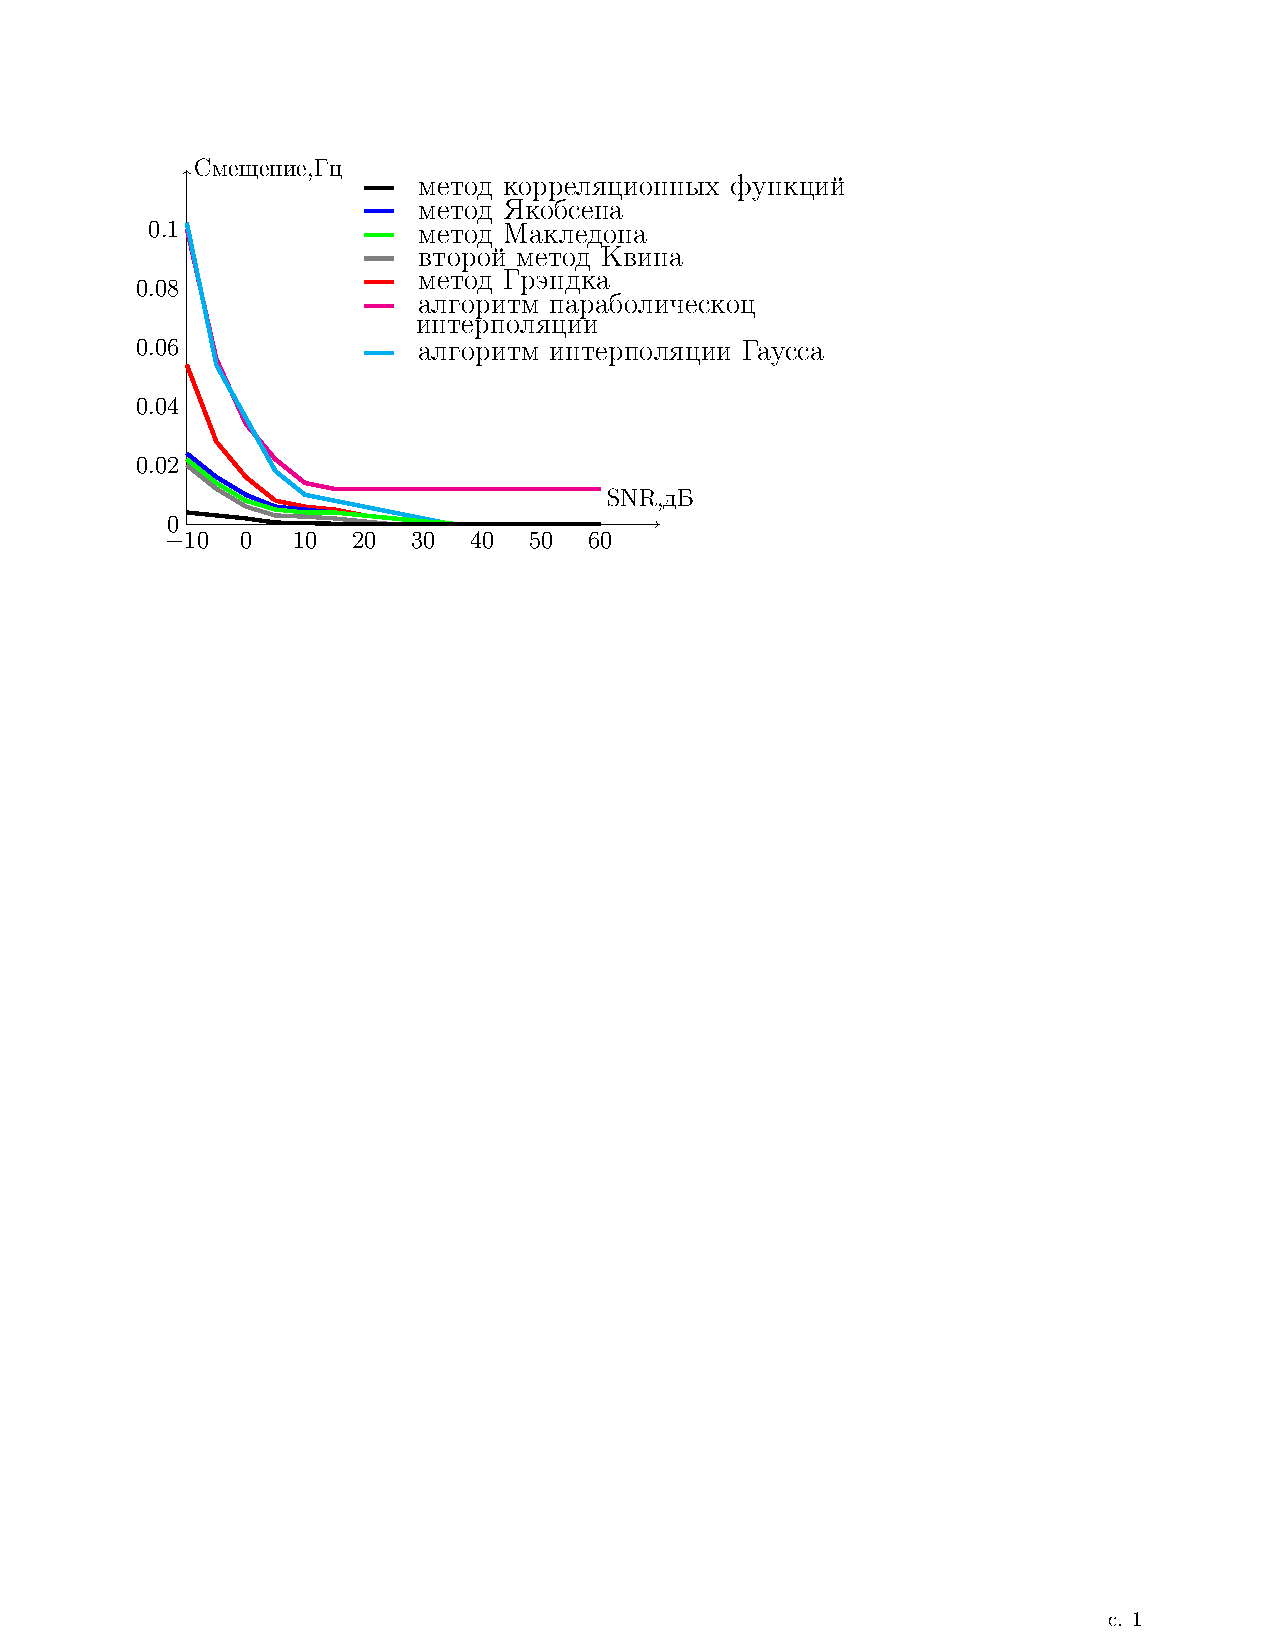
\includegraphics [scale=0.45] {Fundamental frequency offset versus noise level.pdf}
	\caption{Графики зависимостей смещения основной частоты от уровня шума.}
	\label{img:Fundamental_frequency_offset_versus_noise_level}
\end{figure}
\end{tabular}
\end{frame}

%\subsection{Уточнение границы Крамера-Рао}
%\begin{frame}{Оценка дисперсии амплитуды гармоники}
%\textbf{	\textsc{Основные результаты из статьи <<Граница Крамера-Рао для амлитуды гармоники при использовании оконных функций>>}:}
%\begin{itemize}
%\item Оценку точности результатов для данных, которые сами по себе являются оценкой точности, выполнить на прямую довольно затруднительно. Во всех трех экспериментах с увеличением числа опытов экспериментальные кривые сглаживались и становились визуально не отличимые от расчетных данных.
%\item Эксперименты были проведены при различных входных параметрах (число точек, амплитуда, частота и фаза сигналов, дисперсия шума или коэффициент окна). Ни в одном случае не было зафиксировано отклонение результатов эксперимента от результатов, полученных по предложенной формуле.
%\item Таким образом, результаты моделирования алгоритма оценки амплитуды гармоники в условиях шума при наложении оконной функции подтверждают полученные соотношения для оценки дисперсии оценки амплитуды.
%\end{itemize}	
%\end{frame}

\begin{frame}{Экспериментальная проверка формулы для оценки дисперсии}
\begin{tabular}{m{0.30\linewidth}m{0.32\linewidth}m{0.32\linewidth}}
\begin{figure}[ht]
	\centering
	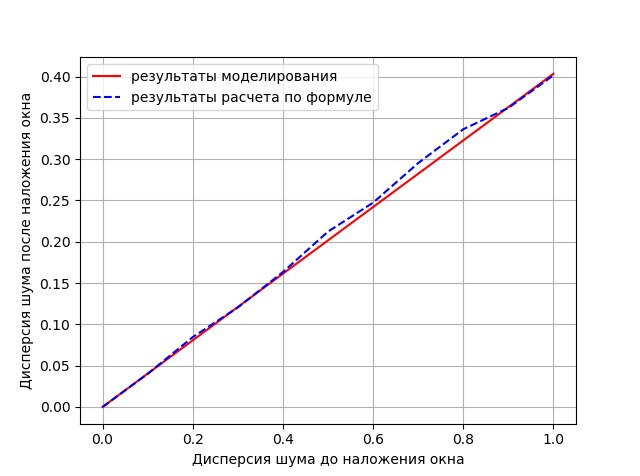
\includegraphics [scale=0.24] {noise_win_var.png}
	\caption{\small{Зависимость дисперсии шума после наложении на него окна.}}
	\label{img:noise_win_var}
\end{figure}
\scriptsize{\begin{equation}
		\label{eq:equation7}
		\sigma^{'2}=\frac{\sum_{n=0}^{N-1} w_n^2}{N}*\sigma^2
\end{equation}}
& 
\begin{figure}[ht]
	\centering
	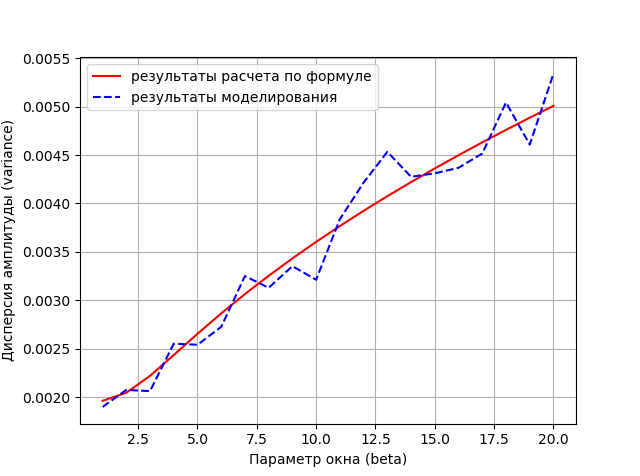
\includegraphics [scale=0.24] {estimate_amp_sin_kaiser_beta.png}
	\caption{\footnotesize{Зависимость дисперсии оценки амплитуды от параметра окна.}}
	\label{img:estimate_amp_sin_kaiser_beta}
\end{figure}
\scriptsize{\begin{equation}
		\label{eq:equation11}
		var(A)\geq \frac{2\sigma^2}{N} \frac{\sum_{n=0}^{N-1}w_n^2}{\left(\sum_{n=0}^{N-1} w_n \right)^2} 			  
\end{equation}}
&
\begin{figure}[ht]
	\centering
	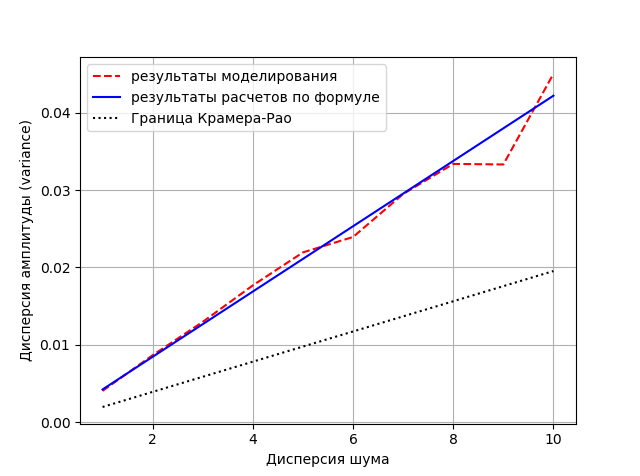
\includegraphics [scale=0.25] {estimate_amp_sin_kaiser_noise.png}
	\caption{\footnotesize{Зависимость дисперсии оценки амплитуды от дисперсии шума.}}
	\label{img:estimate_amp_sin_kaiser_noise}
\end{figure}
\scriptsize{\begin{equation}
		\label{eq:equation11}
		var(A)\geq \frac{2\sigma^2}{N} \frac{\sum_{n=0}^{N-1}w_n^2}{\left(\sum_{n=0}^{N-1} w_n \right)^2} 			  
\end{equation}}
\end{tabular}
\end{frame}

\begin{frame}{Дополненная математическая модель мультигармонического сигнала}
    \begin{center}
		\Large
		Математическая модель мультигармонического сигнала для оценки параметров гармоник
	\end{center}	
	\begin{itemize}
		\item Математическое описание свойств ДПФ.
		\item Математическое описание влияния оконных функций.
		\item \textbf{Формулы для оценки дисперсии результатов измерений}.
	\end{itemize}
\end{frame}

\section{Анализ мультигармонических сигналов}

\subsection{Нахождение гармоники сигнала}
\begin{frame}{Интерполирование спектра}

\scriptsize{
\begin{equation}
	\label{eq:equation3.10}
	A_{\nu} =  \sqrt{\left({\displaystyle\sum_{i=1}^{i=M}\mathrm{Re}(Y_i) \cdot W_{ji}} \right)^2 + \left({\displaystyle\sum_{i=1}^{i=M}\mathrm{Im}(Y_i) \cdot W_{ji}} \right)^2}
\end{equation}
\begin{equation}
	\label{eq:equation3.8.9}
	\varphi = \arctan \left({\frac{\displaystyle\sum_{i=1}^{i=M} \mathrm{Im}(Y_i) \cdot W_{ji}}{\displaystyle\sum_{i=1}^{i=M} \mathrm{Re}(Y_i) \cdot W_{ji}}
	}\right) 
\end{equation}}
\begin{tabular}{m{0.45\linewidth}m{0.45\linewidth}}	
\begin{figure}[ht]
	\centering
	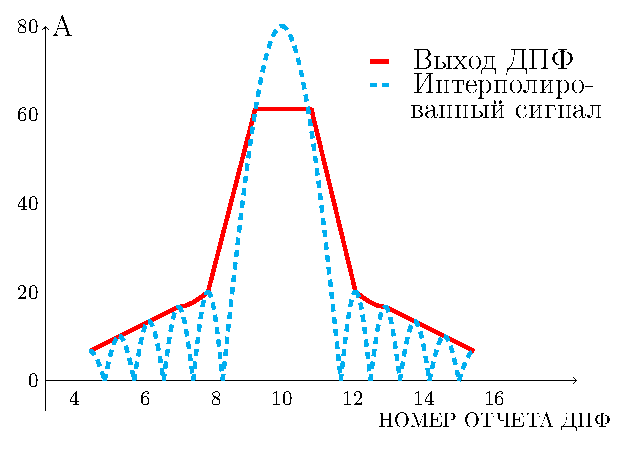
\includegraphics [scale=0.4] {Jacobsen's_method1.pdf}
	\caption{Интерполяция пиков.}
	\label{img:Jacobsen's_method}
\end{figure}
%\textsc{Слева - прямое интерполирование, справа - метод корреляционных функций}
&
\begin{figure}[ht]
	\centering
	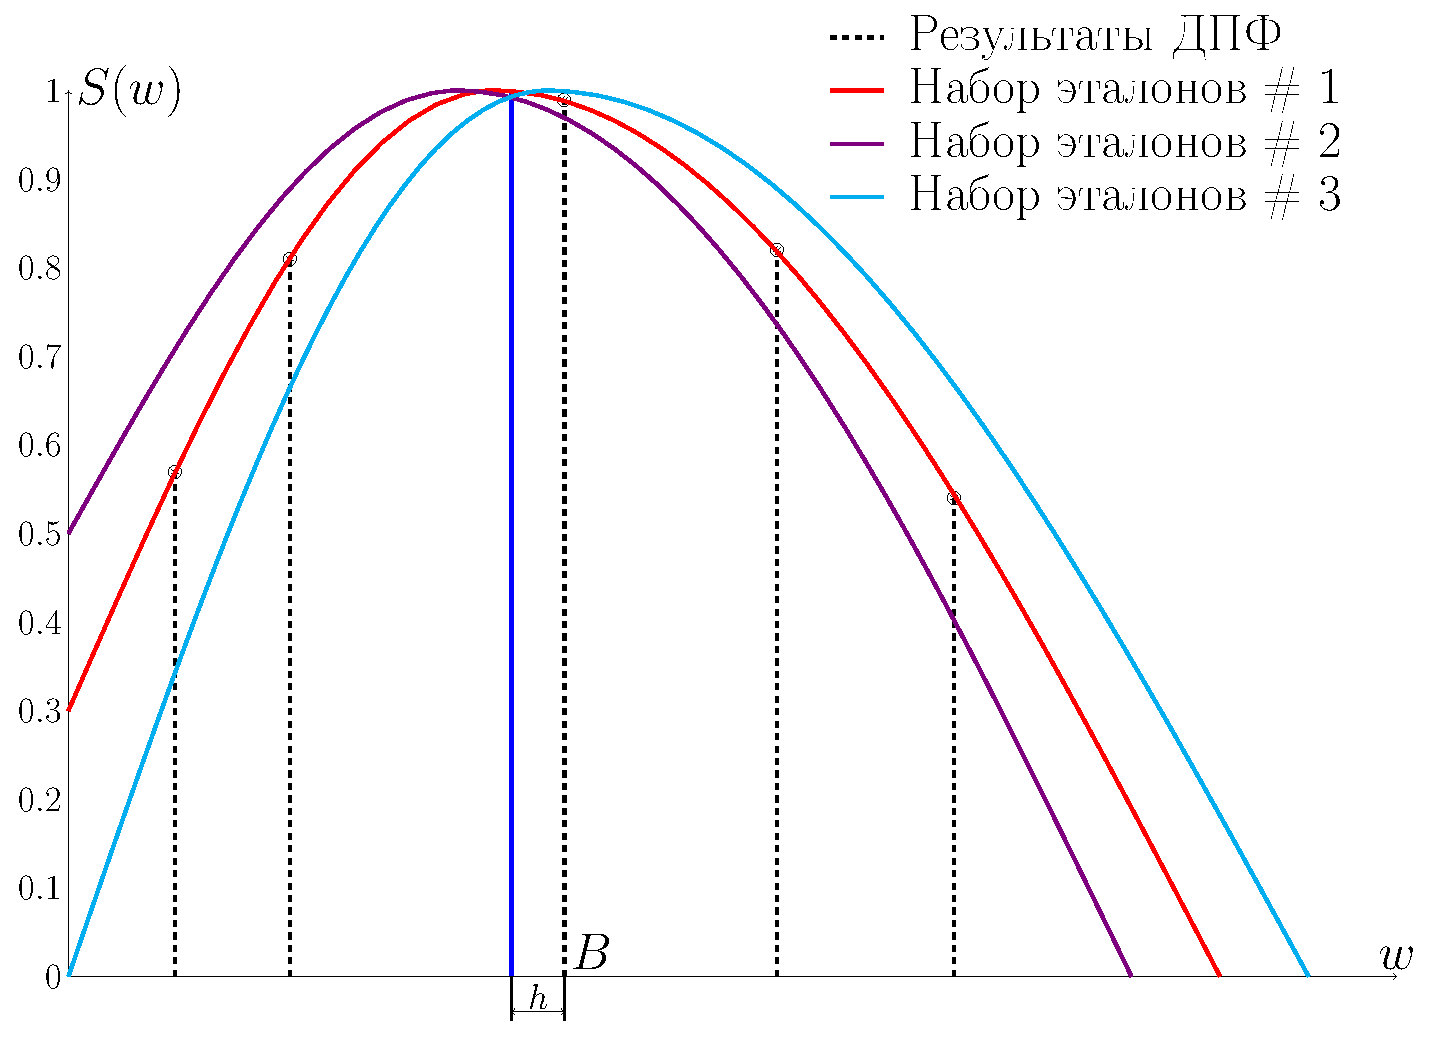
\includegraphics [scale=0.19] {set_of_standards1.pdf}
	\caption{Пример построения наборов эталонов.}
	\label{img:set_of_standards}
\end{figure}	
\end{tabular}
\end{frame}

\begin{frame}{Двойное интерполирование сигнала и спектра}
	\begin{minipage}[t]{0.43\linewidth}
		\centering 
		\textbf{Сигнал (частота=5.2)}
		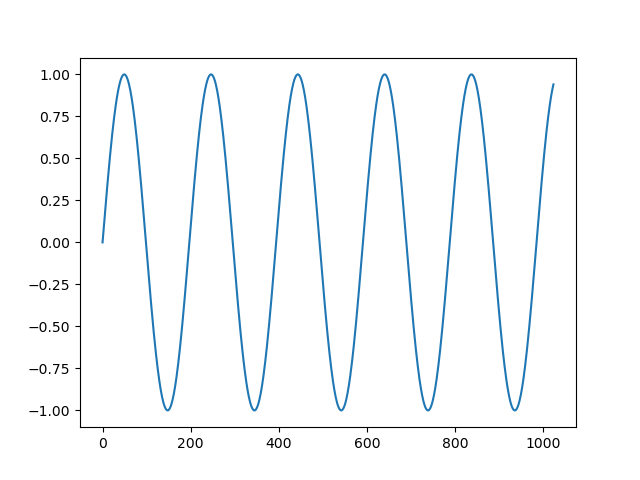
\includegraphics[width=.85\linewidth]{signal}
		\textbf{Экстраполированный \\ сигнал ($k_{i1}=4$)}
		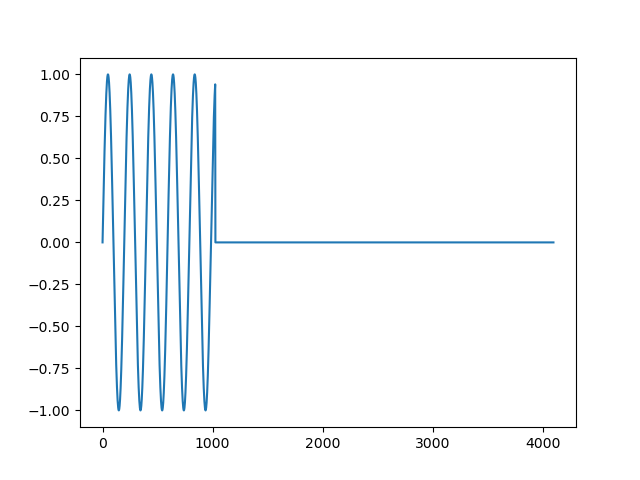
\includegraphics[width=.85\linewidth]{interpolated_signal}		
	\end{minipage}
	\hfill
	\begin{minipage}[t]{0.43\linewidth}
		\centering 
		\textbf{Спектр сигнала}
		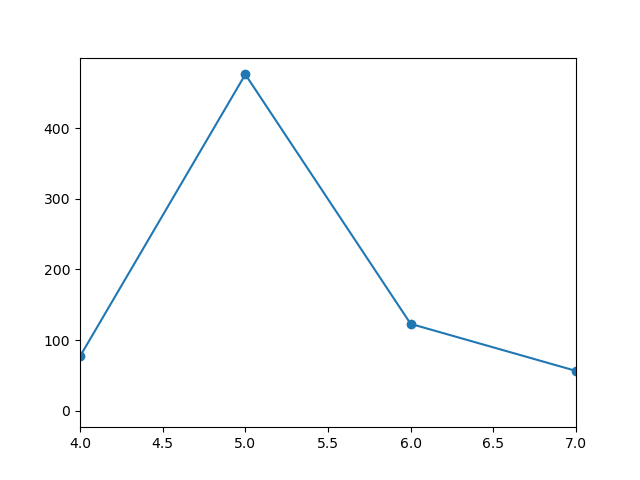
\includegraphics[width=.85\linewidth]{spectrum_double}
		\textbf{Спектр с двойной интерполяцией ($k_{i2}=4$)}
		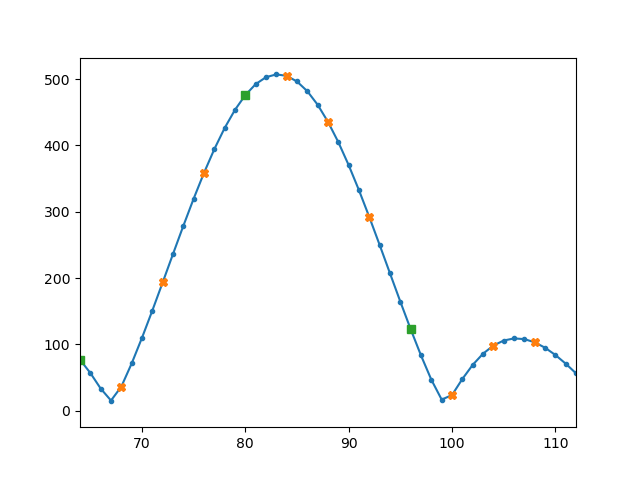
\includegraphics[width=.85\linewidth]{spectrum_double_interpolated}
	\end{minipage}
\end{frame}

\subsection{Поиск гармоник}
\begin{frame}{Алгоритм поиска гармоник}
%	\textsc{ГСА алгоритма поиска гармоник из зарегистрированной программы}
\begin{figure}[ht]
	\centering
	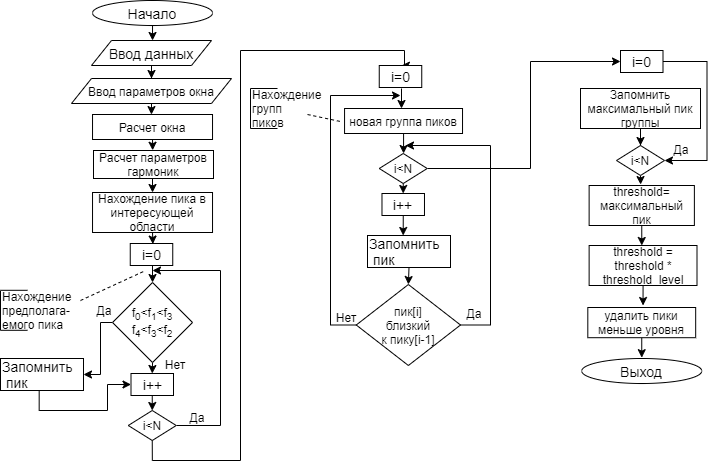
\includegraphics [scale=0.40] {GSA.png}
	\caption{ГСА алгоритма поиска гармоник.}
	\label{img:Diagram_GSA}
\end{figure}
\end{frame}

\begin{frame}{Расчет гармоник и интергармоник}
	\textsc{Свидетельство о регистрации программы}
\begin{tabular}{m{0.45\linewidth}m{0.45\linewidth}}
\begin{figure}[ht]
	\centering
	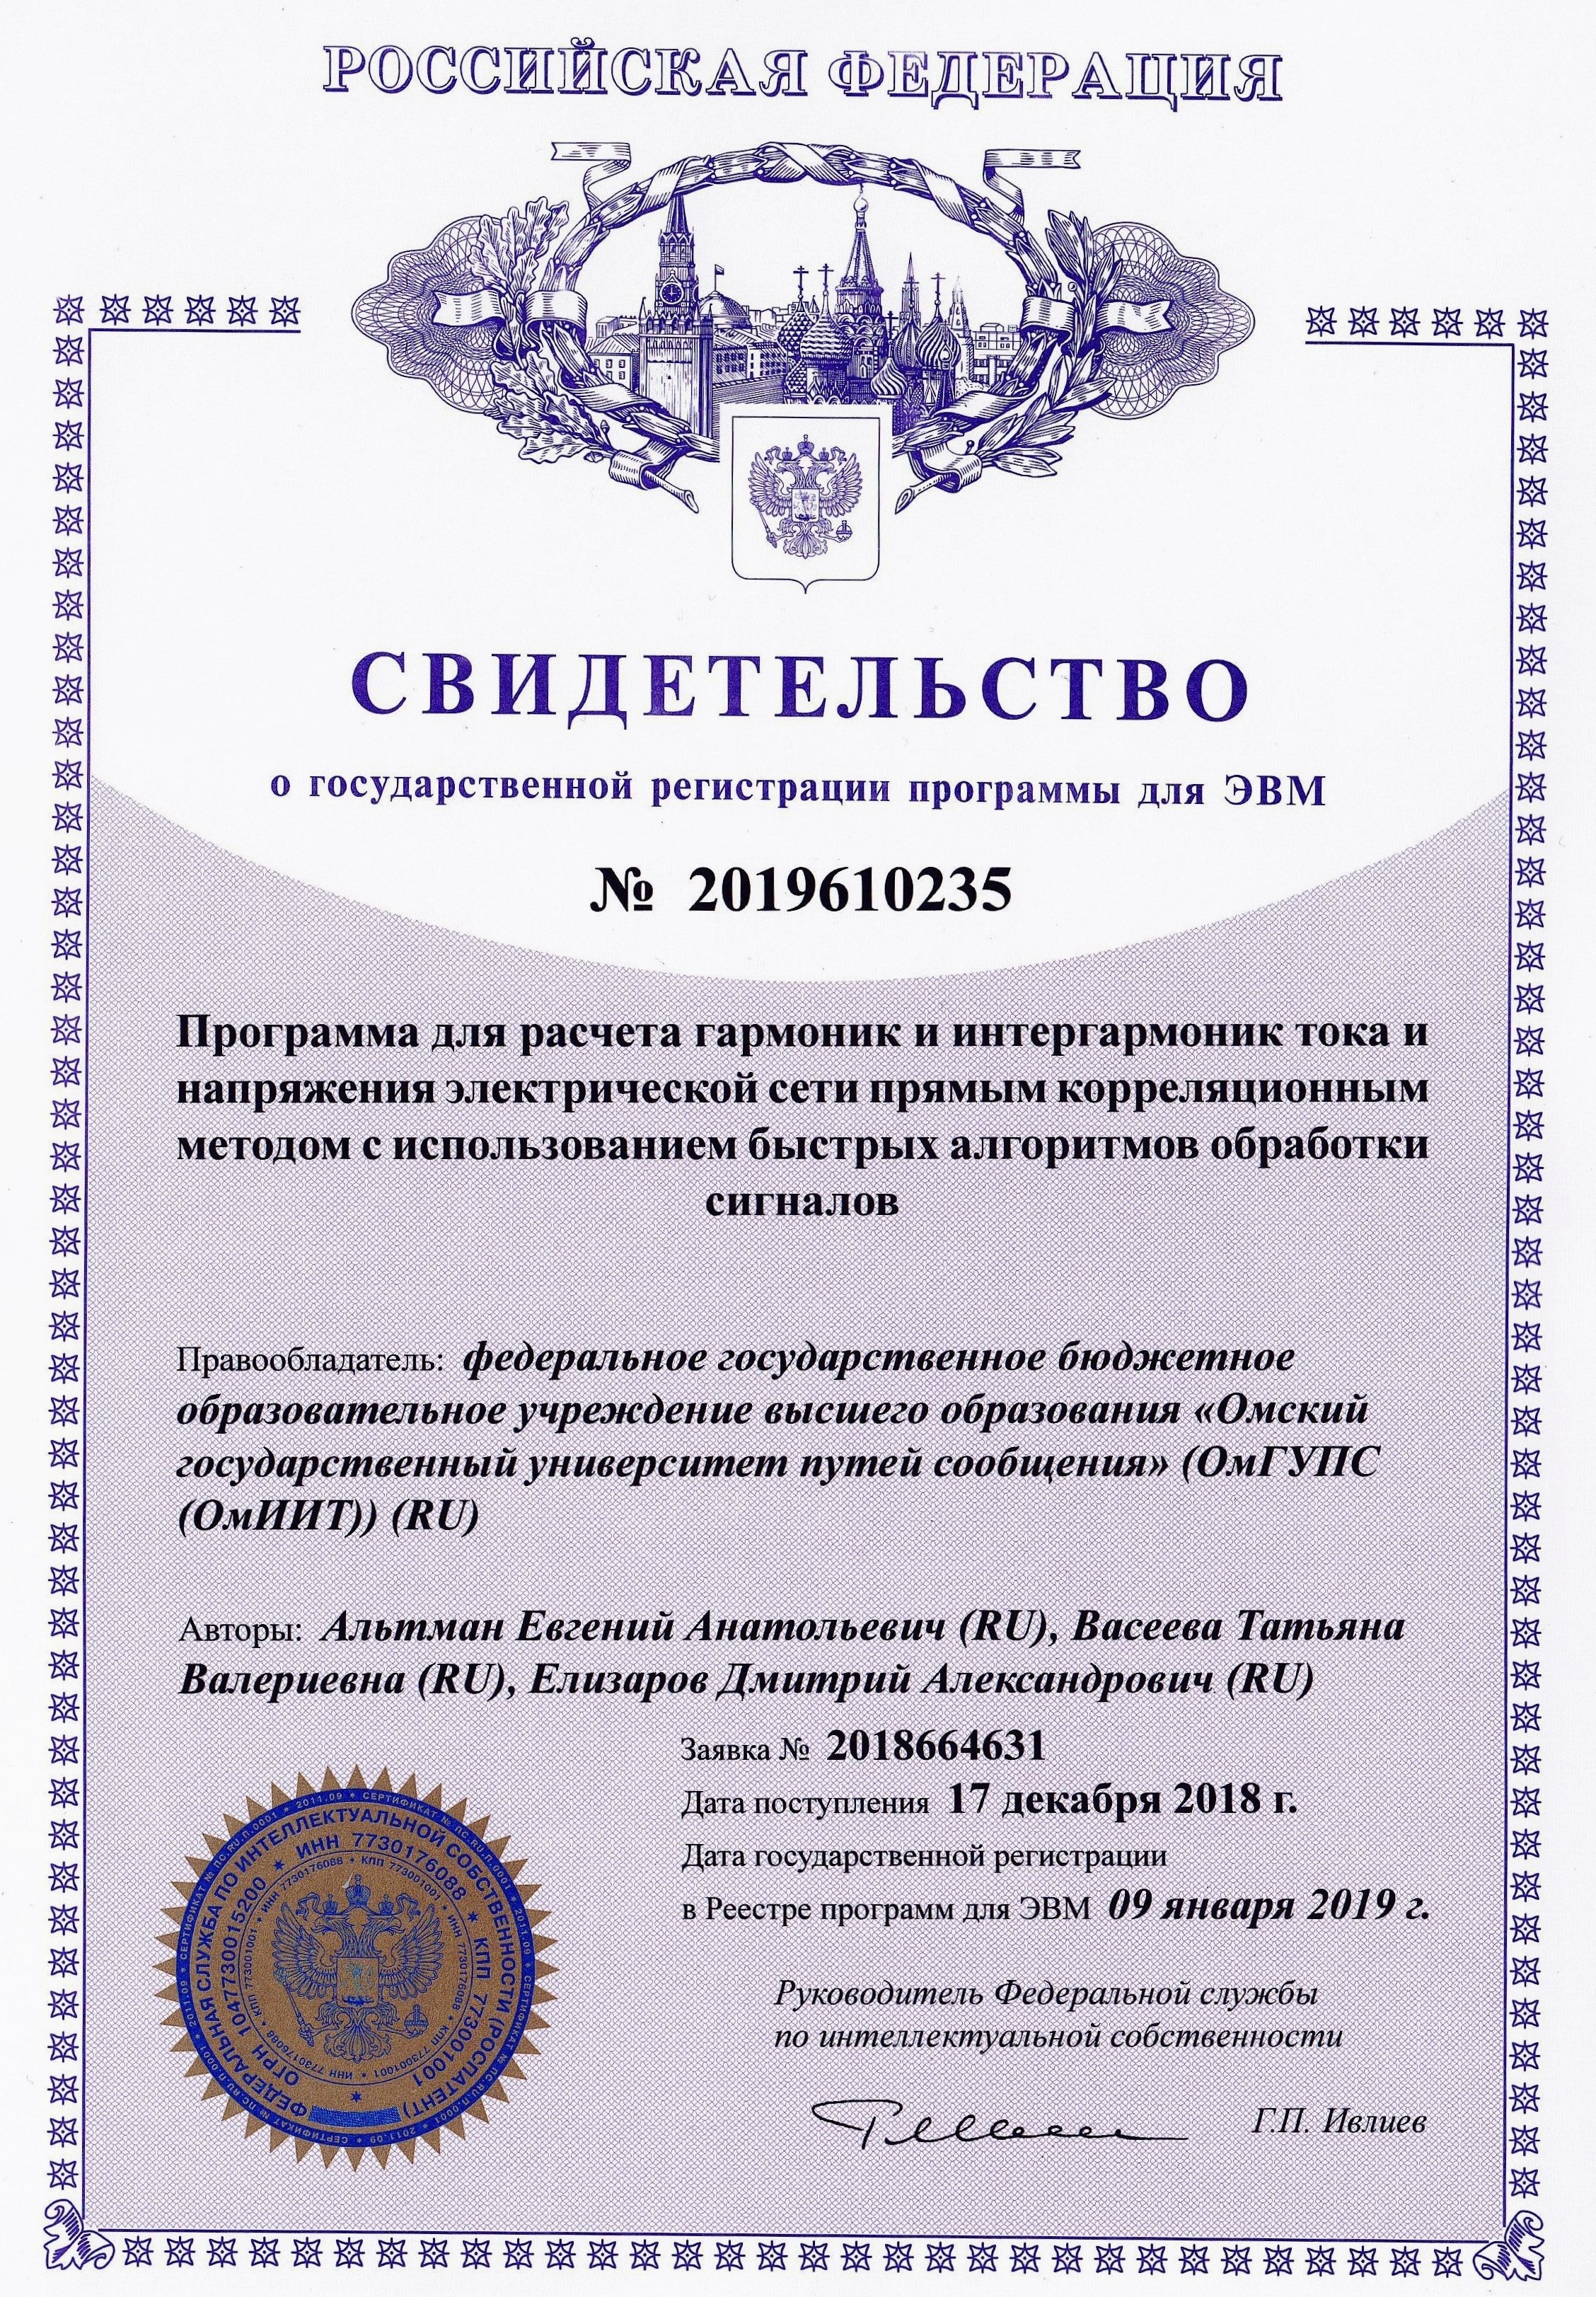
\includegraphics [scale=0.07] {Computer_program1.jpg}
	\caption{Свидетельство.}
	\label{img:Computer_program}
\end{figure}
&
\begin{figure}[ht]
	\centering
	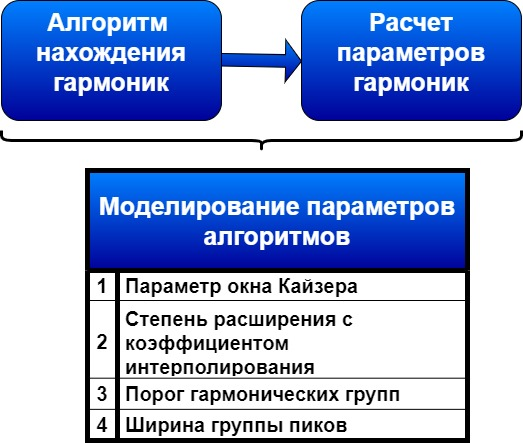
\includegraphics [scale=0.3] {Diagram_Computer_program2.jpg}
	\caption{Функционал в зарегистрированной программе.}
	\label{img:Diagram_Computer_program}
\end{figure}
%Предлагаемая полезная модель относится к электроизмерительной технике и может быть использована для определения гармоник.
\end{tabular}
\end{frame}

\subsection{Практическая реализация}
\begin{frame}{Метод нахождения параметров гармоник}
	\begin{block}{При заданной точности по частоте}
		$k_i=\frac{f_1}{f_{eps}}$, 
		
		${f_{eps}}$ -- заданная точность
	\end{block}	
	\begin{block}{При заданной точности по амплитуде}
		$f_{eps}=a_{eps}*\frac{sw_0-w_1}{sw_0}$,  
		
		$a_{eps}$ -- заданная точность, $sw_i$ -- отсчеты спектра окна.
	\end{block}
	\begin{block}{При заданном шуме}
		$a_{eps} = var(A)\geq \frac{2\sigma^2}{N} \frac{\sum_{n=0}^{N-1}w_n^2}{\left(\sum_{n=0}^{N-1} w_n \right)^2}$ Формула для оценки дисперсии амплитуды
	\end{block}
\end{frame}


\begin{frame}{Использование корреляции}
\begin{tabular}{m{0.45\linewidth}m{0.49\linewidth}}
	\begin{figure}[ht]
		\centering
		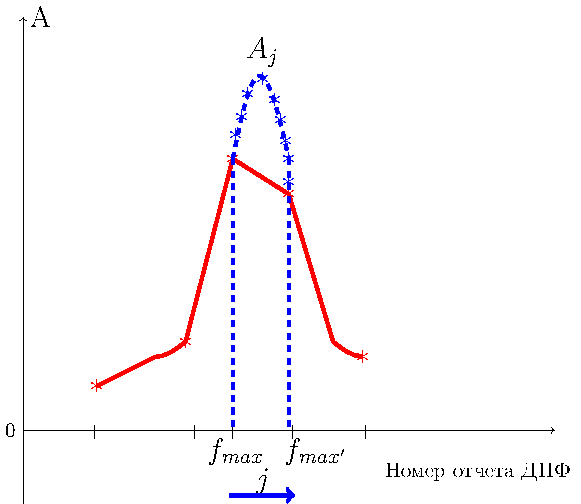
\includegraphics [scale=0.5] {Using_correlation.pdf}
		\caption{Использование корреляции.}
		\label{img:Using_correlation}
	\end{figure}
&
\begin{equation}
\label{eq:equation3.10}
j = 0, 1, \cdots M-1
\end{equation}
\begin{equation}
\label{eq:equation3.10}
f_j = \frac{\left| f_{max}- f_{max'} \right| }{M} + f_{max'}
\end{equation}
\begin{equation}
\label{eq:equation3.10}
A_j = w_j \cdot
\displaystyle\sum_{k=0}^{M-1} x(k) \cdot \exp \left( -i \cdot f_j \cdot \frac{2 \pi k}{N}\right) 
\end{equation}

$f_{max}$ -- частота гармоники ДПФ с наибольшей амплитудой;

$f_{max}'$ -- частота гармоники ДПФ со 2 по величине амплитуде;

$w_j$ -- коэффициент окна;

$j$-ый отсчет спектра окна. 
\end{tabular}
\end{frame}

\begin{frame}{Pruned FFT}
\begin{tabular}{m{0.45\linewidth}m{0.49\linewidth}}
\begin{figure}[ht]
	\centering
	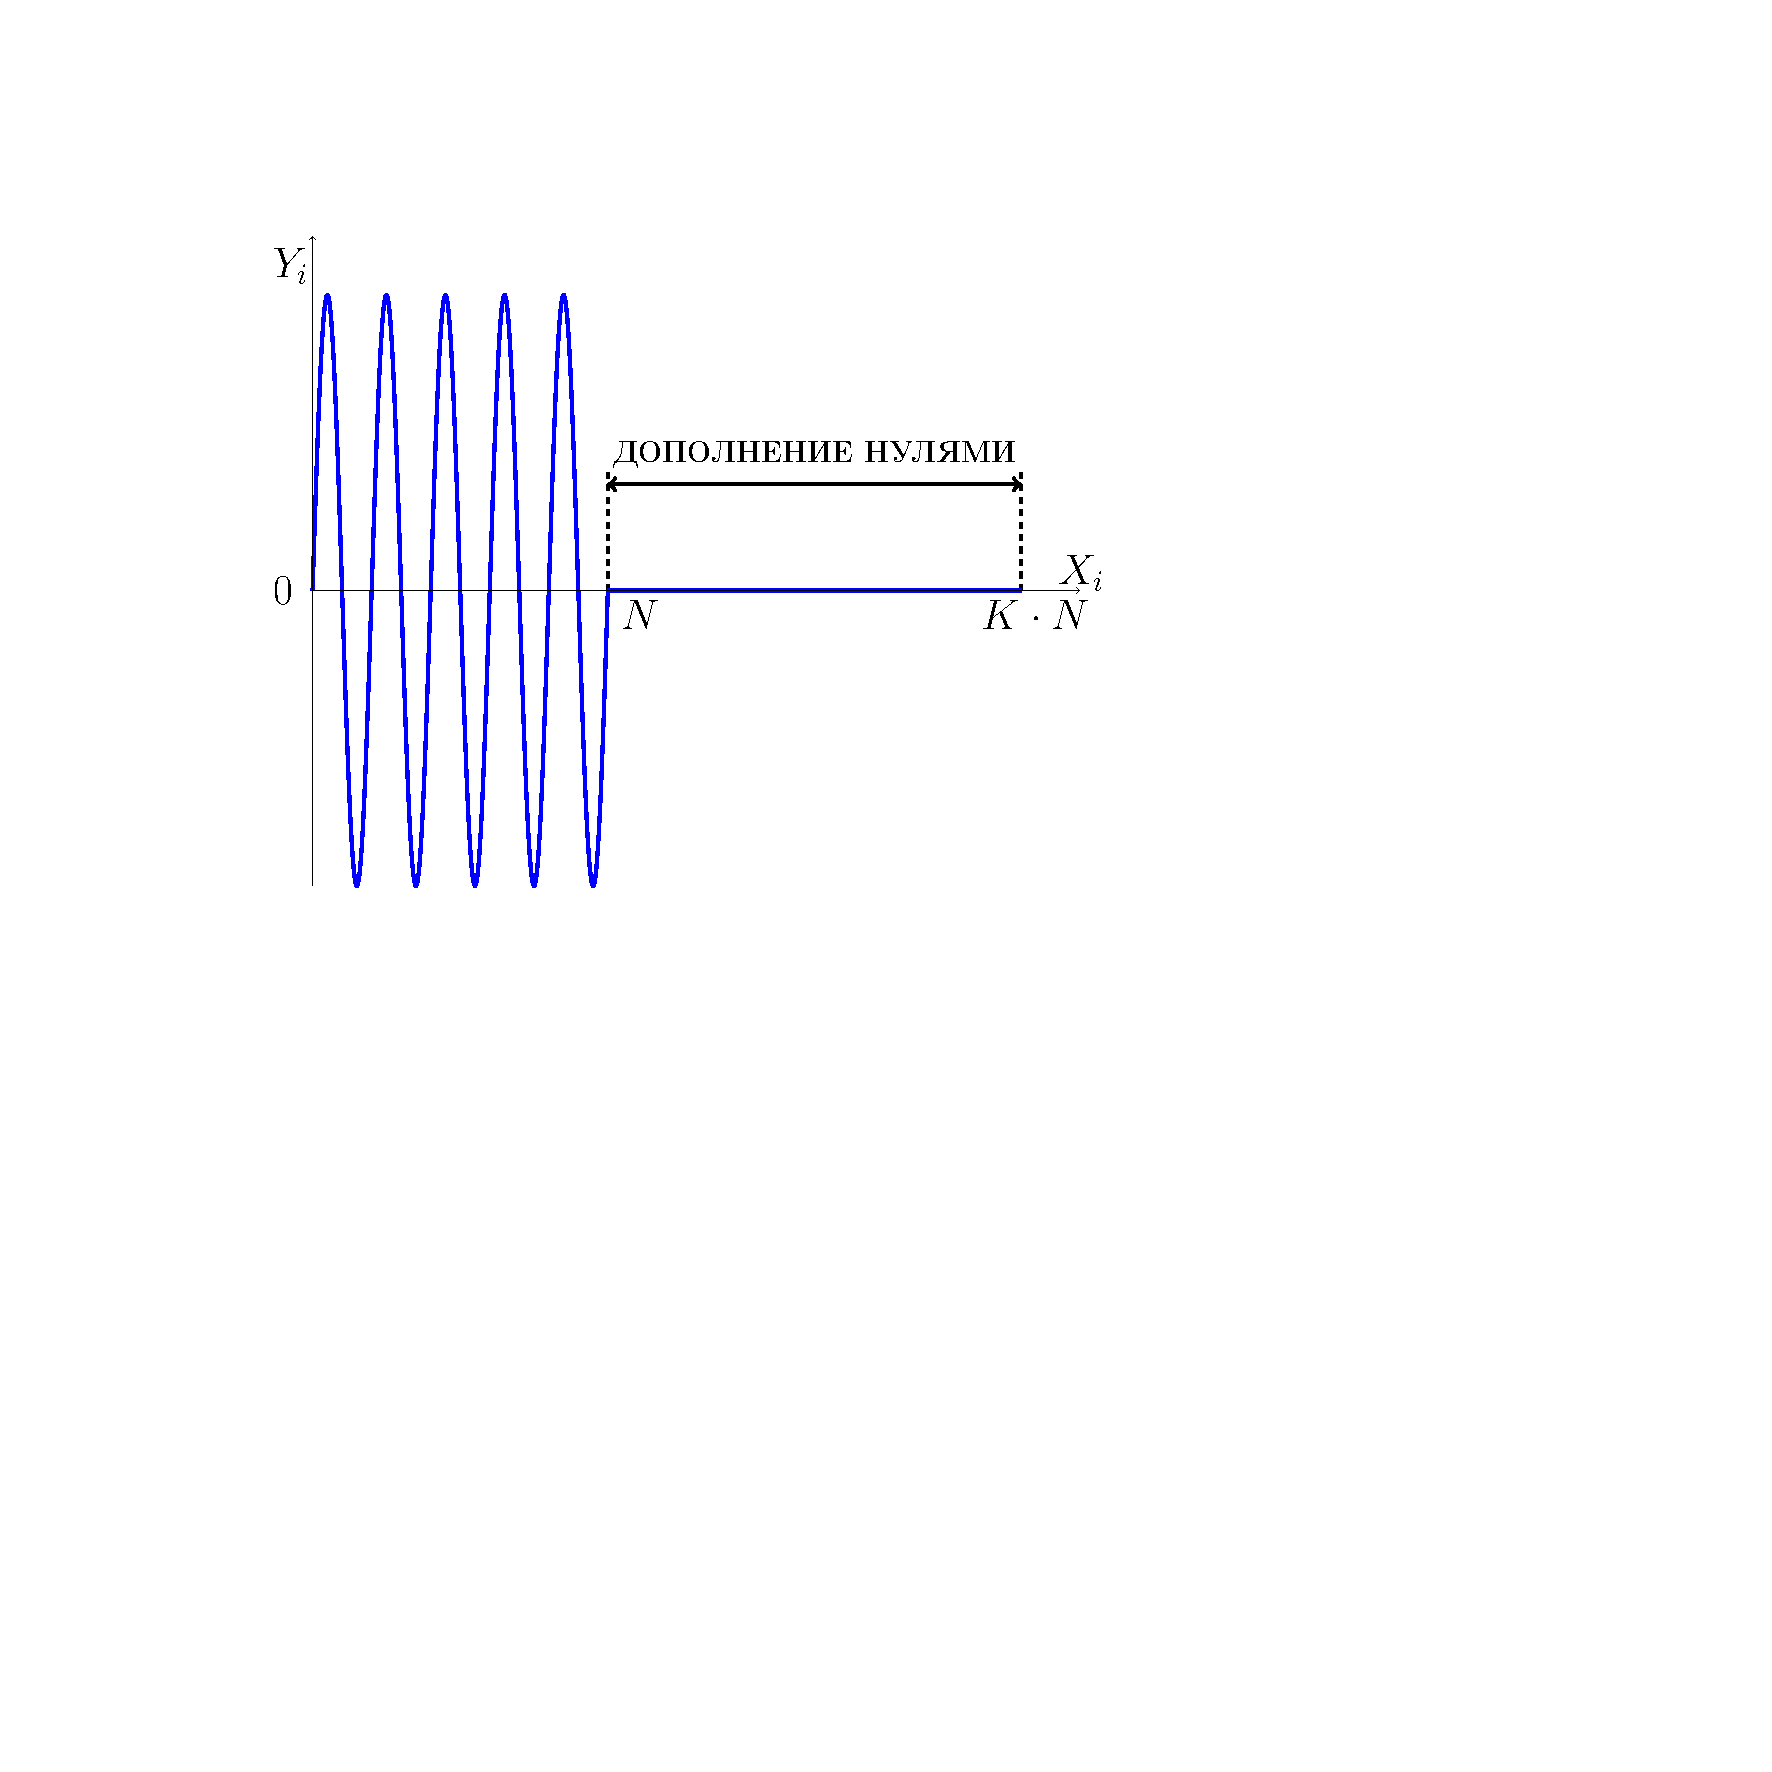
\includegraphics [scale=0.3] {Pruned_FFT.pdf}
	\caption{Исходный сигнал.}
	\label{img:Pruned_FFT}
\end{figure}
\textbf{Матричная форма:}
\tiny{
\begin{center}
	$\longrightarrow N$	
\end{center}
\begin{equation}
\label{eq:equation111}
\downarrow K 
	\begin{pmatrix}
	X_{0} & X_{1} & \cdots & X_{n-1} \\
	X_{N} & X_{n+1} & \cdots & X_{2n-1} \\
	\vdots  & \vdots  & \ddots & \vdots  \\
	X_{N(k-1)} & \cdots & \cdots & X_{N(k-1)} 
	\end{pmatrix}
\Bigg \} {\text{НУЛИ}}
\end{equation}} 
&
\textbf{Обобщаем алгоритм Кули-Тьюки:}
\begin{enumerate}
	\item Вычисляем БПФ столбцов;
	\item Умножаем на поворачивающие множители;
	\item Вычисляем БПФ строк.
\end{enumerate}
\textbf{Pruned FFT}
\begin{itemize}
	\item Не требует $1$-й стадии вычислений;
	\item Сложность алгоритма $N \cdot \log(N) \cdot K$;
	\item Сложность растет линейно с ростом $K$.
\end{itemize}
\end{tabular}
\end{frame}

%\begin{frame}{Анализ быстродействия}
%	\begin{block}{}
%		\begin{minipage}[t]{0.47\linewidth}
%			\centering \textcolor{blue}{\textbf{Прямой метод}}
%			%\textsc{Найти график, желательно с CUDA}	
%			\begin{figure}[ht]
%				\centering
%				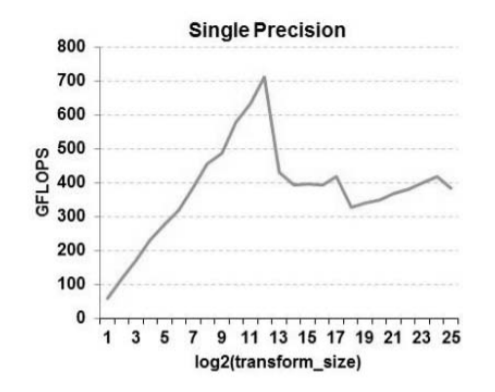
\includegraphics [scale=0.27] {CUDA.PNG}
%				%\caption{CUDA.}
%				\label{img:CUDA}
%			\end{figure}			
%			%\textcolor{blue}{\textit{Не подходит для встроенных систем}}
%		\end{minipage}
%		\begin{minipage}[t]{0.47\linewidth}
%			\centering \textcolor{blue}{\textbf{Sparse FFT}}
%			%\textsc{График с сайта}		
%			\begin{figure}[ht]
%				\centering
%				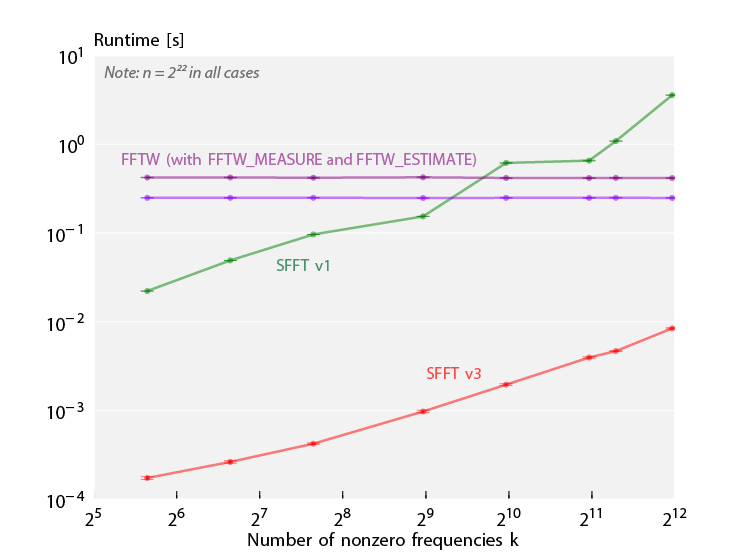
\includegraphics [scale=0.25] {Sparse_Fourier_Transform_Performance.png}
%				%\caption{Sparse FFT.}
%				\label{img:Sparse_Fourier_Transform_Performance}
%			\end{figure}
%			%\textcolor{blue}{\textit{Не работает с интерполированными сигналами}}
%		\end{minipage}
%	\end{block}
%	\hfil
%	\begin{block}{}
%		\begin{minipage}[t]{0.47\linewidth}
%			\centering \textcolor{blue}{\textbf{Быстрая корреляция}}
%			%\textsc{Найти график}	
%			\begin{figure}[ht]
%				\centering
%				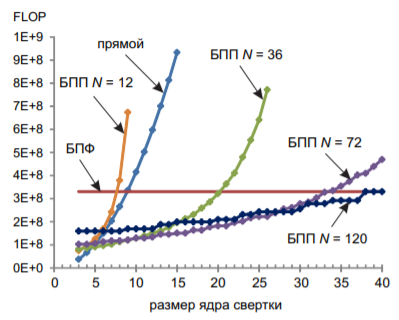
\includegraphics [scale=0.3] {Прямая_корреляция2.PNG}
%				%\caption{Быстрая корреляция.}
%				\label{img:Прямая_корреляция}
%			\end{figure}			
%			%\textcolor{blue}{\textit{Высокое быстродействие при малом коэффициенте интерполирования}}	
%		\end{minipage}
%		\begin{minipage}[t]{0.47\linewidth}
%			\centering \textcolor{blue}{\textbf{Pruned БПФ}}
%			%\textsc{Найти график}	
%			\begin{figure}[ht]
%				\centering
%				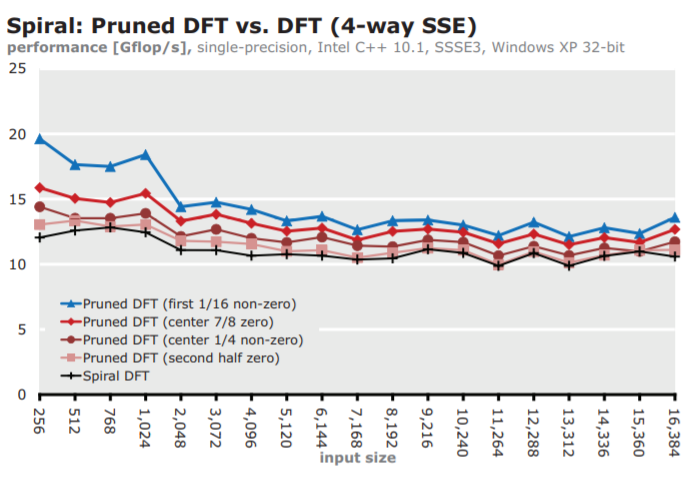
\includegraphics [scale=0.25] {Pruned_DFT.PNG}
%				%\caption{Pruned БПФ.}
%				\label{img:Pruned_DFT}
%			\end{figure}			
%			%\textcolor{blue}{\textit{Относительно высокое быстродействие, слабо зависит от коэффициента интерполирования}}	
%		\end{minipage}
%	\end{block}
%\end{frame}

\begin{frame}{Анализ быстродействия}
	\begin{minipage}[t]{0.45\linewidth}
	\centering 
	\textbf{Быстрая корреляция}
	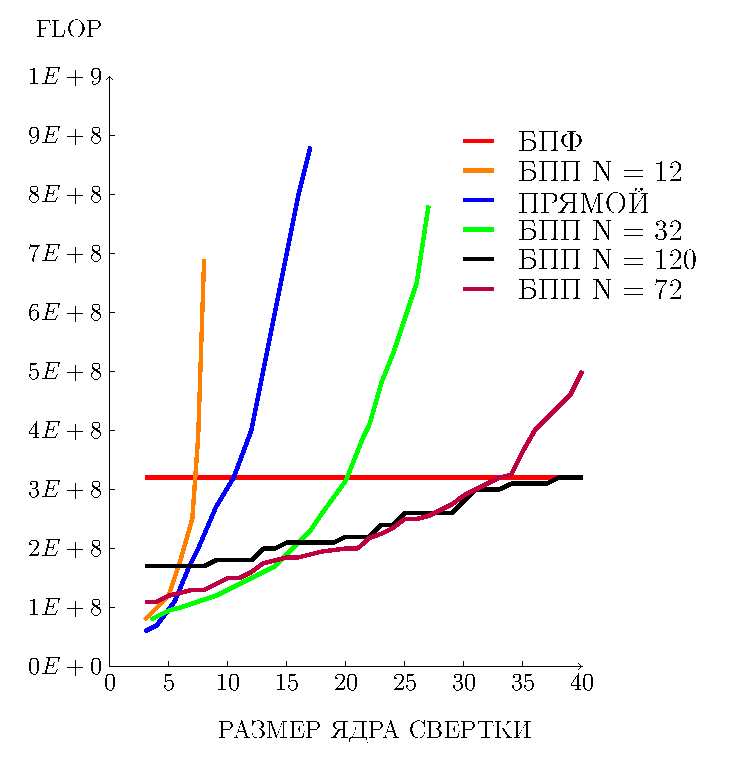
\includegraphics[width=.745\linewidth]{Direct correlation.pdf}
	\textbf{Pruned БПФ}
	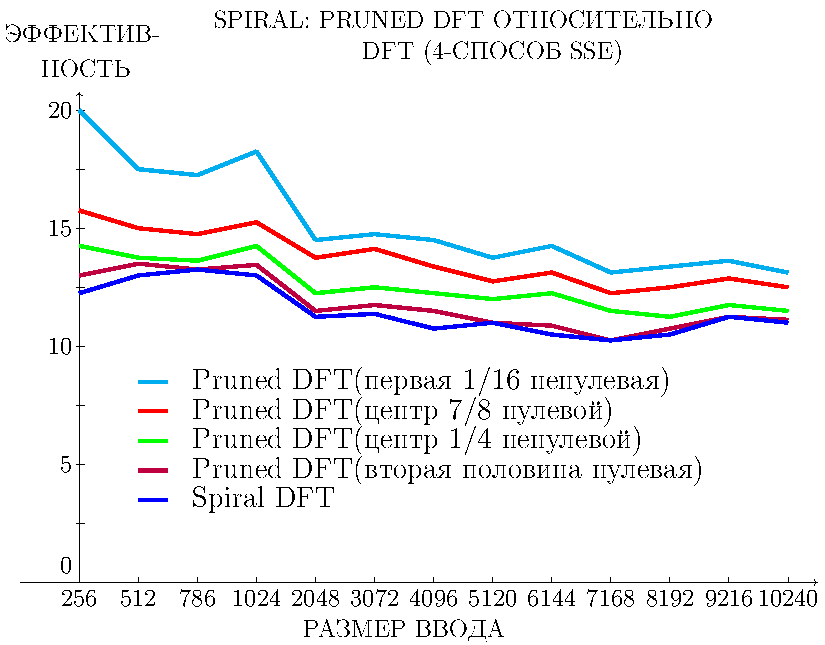
\includegraphics[width=.745\linewidth]{Pruned DFT2.pdf}		
\end{minipage}
\hfill
\begin{minipage}[t]{0.45\linewidth}
	\centering 
	\textbf{Прямой метод}
	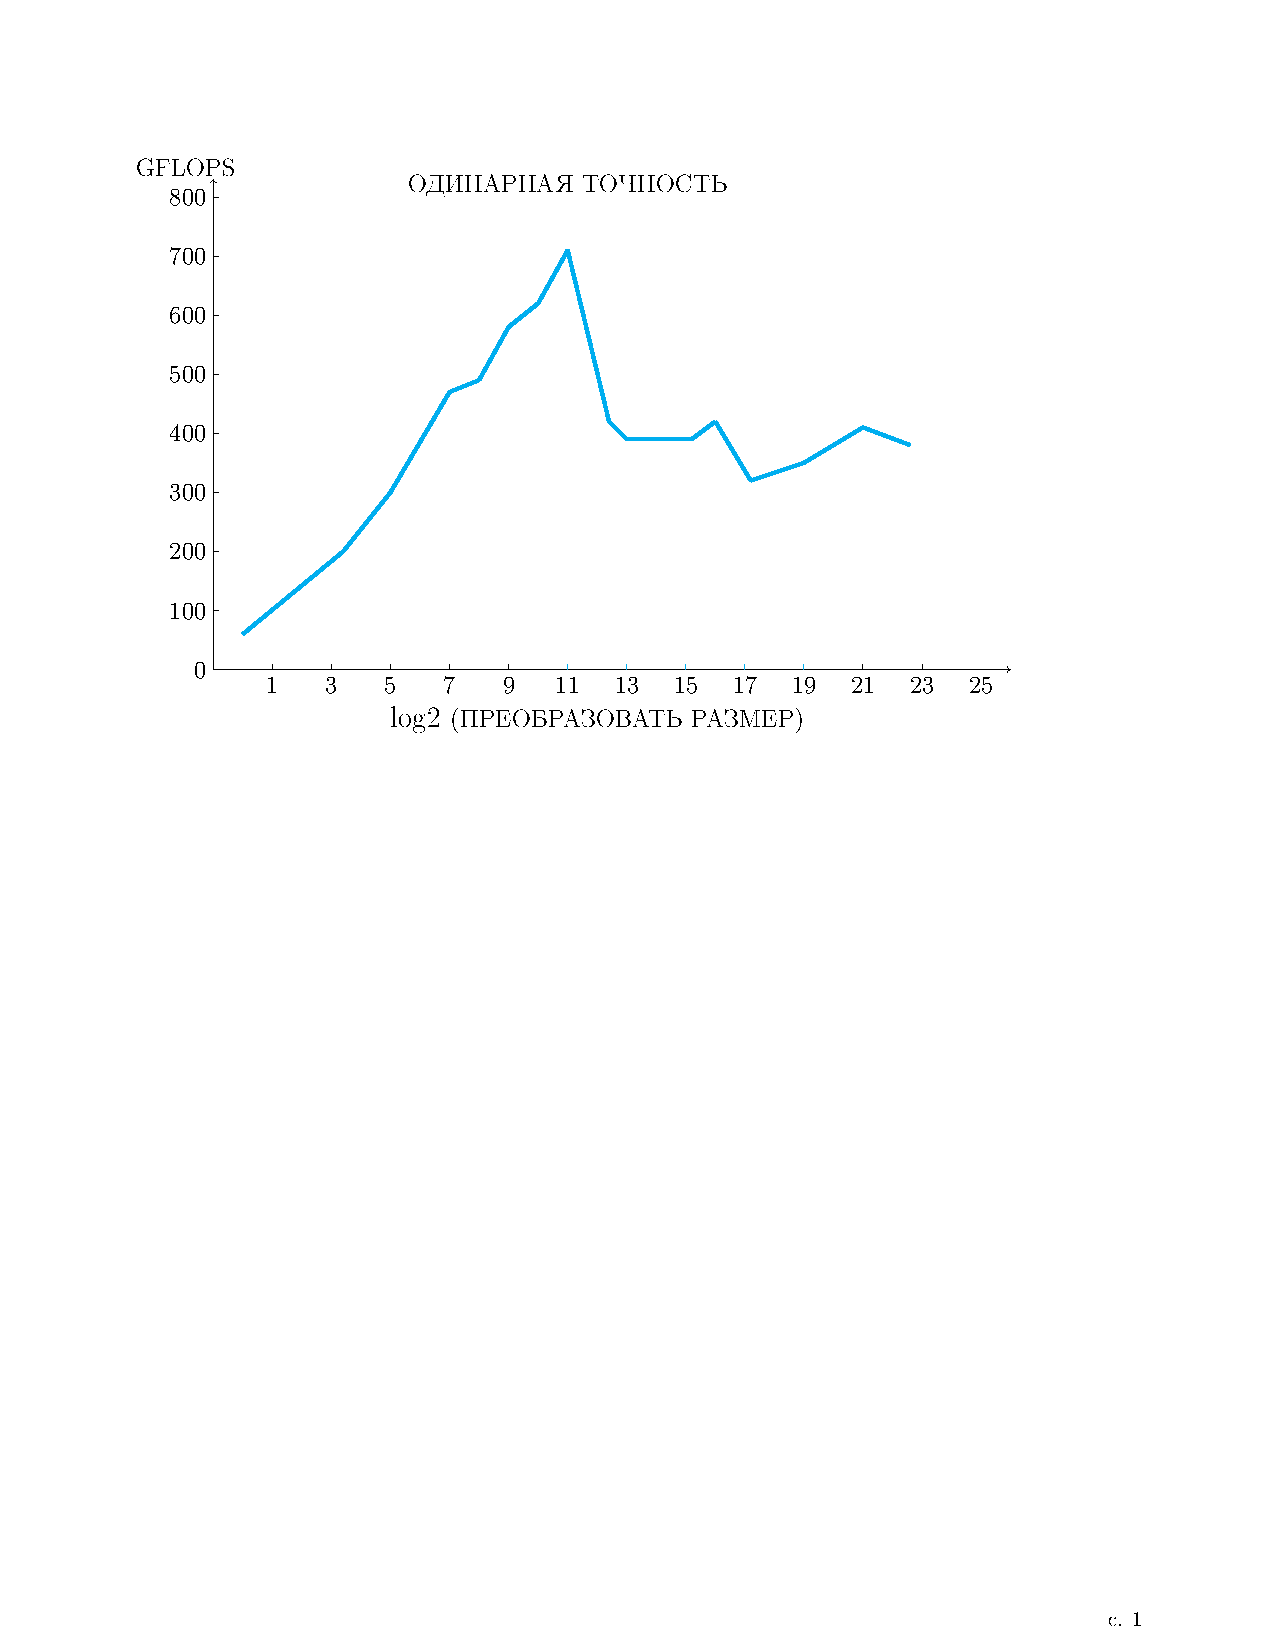
\includegraphics[width=.9\linewidth]{CUDA.pdf}
	\textbf{Sparse FFT}
	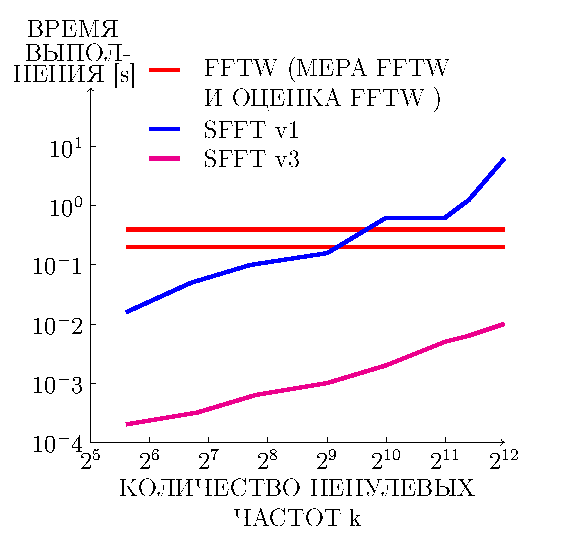
\includegraphics[width=.8\linewidth]{Sparse Fourier Transform2.pdf}
\end{minipage}
\end{frame}



\section{Заключение}

\subsection{Результаты работы}
\begin{frame}{Список опубликованных работ}
\scriptsize{
\textbf{В изданиях из перечня ВАК Минобрнауки России:}	
\begin{itemize}
	\item Альтман Е.~А., Захаренко Е.~И., Васеева Т.~В. Применение метода разложения двумерной свертки при реализации цифровых фильтров // Научный вестник Новосибирского государственного технического университета. – $2017$. – \textnumero.~$4$. – С. $95$-$104$.
	
	\item Лаврухин А.~А., Малютин А.~Г., Васеева Т.~В. Повышение эффективности информационно-измерительного комплекса автоматизированной системы мониторинга и учета электроэнергии // Известия Транссиба. – $2018$. – \textnumero.~$4 (36)$.
\end{itemize}}	
\scriptsize{
\textbf{SCOPUS:}	
\begin{itemize}
	\item Altman E.~A., Vaseeva T.~V., Aleksandrov A.~V. Cache-aware algorithm for multidimensional correlations //Journal of Physics: Conference Series. – IOP Publishing, $2019$. – Т. $1260$. – \textnumero.~$4$. – С. $042001$.
	
	\item Altman E.~A., Vaseeva T.~V., Aleksandrov A.~V. The derivation Cramer-Rao lower bound for parameters of signals multiplied on window functions //Journal of Physics: Conference Series. – IOP Publishing, 2021. – Т. $1791$. – \textnumero. $1$. – С. $012067$.
\end{itemize}}

\normalsize{Основные результаты по теме диссертации изложены в \textbf{25} печатных изданиях, \textbf{2} из которых изданы в журналах, рекомендованных ВАК, \textbf{2} -- в периодических научных журналах, индексируемых Web of Scopus, \textbf{17} -- в тезисах докладах, \textbf{4} отчетах НИР, \textbf{1} свидетельство о регистрации программы для ЭВМ}


%\scriptsize{
%\textbf{В прочих изданиях:}
%\begin{itemize}
%	\item Васеева, Т.~В. Граница Крамера-Рао амплитуды однотонального сигнала для методов ее оценки с использованием оконных функций / Т.~В. Васеева, Е.~А. Альтман //Инновационные проекты и технологии в образовании, промышленности и на транспорте. – $2021$. – С. $301$-$307$.
%	
%	\item Васеева Т.~В., Альтман Е.~А., Александров А.~В. Cравнительное исследование гармонических и интергармонических методов оценки сигналов //Инновационные проекты и технологии в образовании, промышленности и на транспорте. – $2020$. – С. $51$-$57$.
%		
%	\item Малютин А.~Г. и др. Математическое моделирование и численные методы для исследования алгоритмов обработки сигналов и анализа систем массового обслуживания. – $2020$.
%\end{itemize}}
\end{frame}	

%\begin{frame}{Результаты работы}
%\scriptsize{
%\begin{itemize}
%	\item Альтман Е.~А., Васеева Т.~В., Александров А.~В. Граница Крамера-Рао для амплитуды гармоники при использовании оконных функций // Динамика систем, механизмов и машин. – $2020$. – Т. $8$. – \textnumero.~$2$. – С. $145$-$152$.
%	
%	\item Малютин А.~Г. и др. Математическое моделирование, численные методы и комплексы программ для решения задач обработки сигналов и измерения характеристик технических систем. – $2019$.
%	
%	\item  Малютин А.~Г. и др. Совершенствование подходов, архитектур и алгоритмов информационно-управляющих систем и средств измерения. – $2019$.
%		
%	\item Альтман Е.~А., Васеева Т.~В., Александров А. В. Оценка сложности алгоритма БПФ при моделировании его работы // Инновации в информационных технологиях, машиностроении и автотранспорте. – $2019$. – С. $116$-$118$.
%	
%	\item Альтман Е.~А., Александров А.~В., Васеева Т.~В. Современные информационные технологии разработки программ для обработки радиотехнических сигналов на примере БПФ // Надежность функционирования и информационная безопасность инфокоммуникационных, телекоммуникационных и радиотехнических сетей и систем. – $2019$. – С. $132$-$139$.
%	
%	\item Васеева Т.~В., Альтман Е.~А., Елизаров Д.~А. Сравнительный анализ методов определения параметров гармоник сигнала электрической сети // Инновационные проекты и технологии в образовании, промышленности и на транспорте. – $2019$. – С. $261$-$267$.
%
%	\item Васеева Т.~В., Альтман Е.~А., Александров А.~В. Сравнительный анализ применения алгоритмов определения частоты при оценке гармоник в электрических сетях // Системы управления, информационные технологии и математическое моделирование. – $2019$. – С. $61$-$66$.
%\end{itemize}}
%\end{frame}

%\begin{frame}{Результаты работы}
%\scriptsize{
%\begin{itemize}
%	\item Альтман Е.~А., Васеева Т.~В., Александров А.~В. Кэш-ориентированный алгоритм для вычисления многомерной корреляции // Проблемы машиноведения. – $2019$. – С. $385$-$389$.
%	
%	\item Малютин А. Г. и др. Математическое моделирование, численные методы и комплексы программ для решения задач обработки сигналов и анализа структуры информационной системы. – 2018.
%	
%	\item Васеева Т.~В., Альтман Е.~А., Малютин А.~Г. Применение быстрых алгоритмов для выполнения фильтрации изображений // Современные проблемы радиоэлектроники. – $2018$. – С. $162$-$165$.
%	
%	\item Альтман Е.~А., Афанасьева Н.~С., Васеева Т.~В. Расширение глубины резкости изображений программным способом // Инновационные проекты и технологии в образовании, промышленности и на транспорте. – $2018$. – С. $222$-$227$.
%	
%	\item Васеева Т.~В., Альтман Е.~А. Исследование точности математических моделей алгоритмов реализованных на языках высокого уровня // Информационные и управляющие системы на транспорте и в. – $2018$. – С. $236$.
%	
%	\item Александров А.~А., Васеева Т.~В., Ананьева Н.~Г. Оценка эффективности алгоритма корреляции для различных аппаратных платформ // Тезисы $XIX$ Всероссийской конференции молодых учёных по математическому моделированию и информационным технологиям. – $2018$. – С. $54$-$54$.
%	
%	\item Васеева Т.~В., Альтман Е.~А., Елизаров Д.~А. Информационно-измерительная система для анализа гармоник сигнала в электрической сети // САПР и моделирование в современной электронике. – $2018$. – С. $131$-$135$.	
%\end{itemize}}
%\end{frame}

%\begin{frame}{Результаты работы}
%\scriptsize{
%\begin{itemize}
%	\item Васеева Т.~В., Александров А.~В. Реализация алгоритмов вычисления корреляции для диагностирования подвижного состава методами корреляционного анализа // Технологическое обеспечение ремонта и повышение динамических качеств железнодорожного подвижного состава. – $2017$. – С. $138$-$142$.
%	
%	\item Терентьева А.~В., Васеева Т.~В., Кильдибеков А.~Б. Алгоритм детектирования лиц в различных ракурсах и наклонах // Инновационные проекты и технологии в образовании, промышленности и на транспорте. – $2017$. – С. $250$-$255$.
%	
%	\item Васеева Т.~В., Альтман Е.~А. Распознавание границ движущихся объектов методами компьютерного зрения // Информационно-телекоммуникационные системы и технологии. – $2017$. – С. $304$-$306$.
%	
%	\item Альтман Е.~А., Васеева Т.~В., Кузнецов Д.~И. Моделирование алгоритмов обработки сигналов с целью оптимизации их аппаратной реализации // Современные научные исследования и разработки. – $2017$. – \textnumero.~$4$. – С. $27$-$29$.	
%	
%	\item Альтман Е.~А., Дикаревич Н.~С., Васеева Т.~В. Детекторы локальных особенностей в системах компьютерного зрения, применяемых на железнодорожном транспорте // Инновационные проекты и технологии в образовании, промышленности и на транспорте. – $2016$. – С. $272$-$280$.
%\end{itemize}}
%\end{frame}

\subsection{Основные положения, выносимые на защиту}
\begin{frame}{Основные положения выносимые на защиту}
\begin{block}{}
	\textbf{1.} Произвели обзор методов: интерполирование спектра (метод Якобсена, два метода Квина, два метода Маклеода, метод Грэндка, алгоритм параболической интерполяции, алгоритм интерполяции Гаусса), алгоритм, рекомендованный в ГОСТ $30804.4.7-2013$, метод корреляционных  функций, Модернизированный метод корреляционных функций, алгоритм вычисления одномерной корреляции, алгоритм вычисления двумерной корреляции, алгоритм дискретного преобразования Фурье (ДПФ), алгоритма быстрого преобразования Фурье (БПФ), алгоритм разряженного преобразования Фурье (Spare FFT). 
\end{block} 
 
	\textbf{2.} Выведена формула для нахождения границы Крамера-Рао при применении оконной функции, которая позволяет повысить эффективность научных исследований различных алгоритмов обработки сигналов с применением оконных функций, заменив моделирование алгоритма с применением различных окон расчетом по предложенной формуле.
\end{frame}

\begin{frame}{Основные положения выносимые на защиту}
	\textbf{3.} Предложенный численный метод, вместе с его быстрой реализацией, позволяют повысить точность и достоверность результатов измерительных приборов для электрических сетей. Численный метод позволяет находить оптимальную несмещенную оценку параметров гармоник.

	\textbf{4.} Разработанный комплекс программ позволяет проводить научные исследования в области цифровой обработки сигналов и используется в учебном процессе: программа прямого корреляционного метода с использованием быстрых алгоритмов обработки сигналов, оценка дисперсии белого шума после наложения на него окна, оценка амплитуды при использовании различных окон, оценка амплитуды при различных уровнях шума, алгоритм вычисления одномерной свертки.
\end{frame}